\documentclass[ignorenonframetext,]{beamer}
\setbeamertemplate{caption}[numbered]
\setbeamertemplate{caption label separator}{: }
\setbeamercolor{caption name}{fg=normal text.fg}
\beamertemplatenavigationsymbolsempty
\usepackage{lmodern}
\usepackage{amssymb,amsmath}
\usepackage{ifxetex,ifluatex}
\usepackage{fixltx2e} % provides \textsubscript
\ifnum 0\ifxetex 1\fi\ifluatex 1\fi=0 % if pdftex
  \usepackage[T1]{fontenc}
  \usepackage[utf8]{inputenc}
\else % if luatex or xelatex
  \ifxetex
    \usepackage{mathspec}
  \else
    \usepackage{fontspec}
  \fi
  \defaultfontfeatures{Ligatures=TeX,Scale=MatchLowercase}
\fi
\usetheme[]{AnnArbor}
\usecolortheme{beaver}
\usefonttheme{structurebold}
% use upquote if available, for straight quotes in verbatim environments
\IfFileExists{upquote.sty}{\usepackage{upquote}}{}
% use microtype if available
\IfFileExists{microtype.sty}{%
\usepackage{microtype}
\UseMicrotypeSet[protrusion]{basicmath} % disable protrusion for tt fonts
}{}
\newif\ifbibliography
\hypersetup{
            pdftitle={Labo 5: Paramètres de dispersion},
            pdfauthor={Visseho Adjiwanou, PhD.},
            pdfborder={0 0 0},
            breaklinks=true}
\urlstyle{same}  % don't use monospace font for urls
\usepackage{color}
\usepackage{fancyvrb}
\newcommand{\VerbBar}{|}
\newcommand{\VERB}{\Verb[commandchars=\\\{\}]}
\DefineVerbatimEnvironment{Highlighting}{Verbatim}{commandchars=\\\{\}}
% Add ',fontsize=\small' for more characters per line
\usepackage{framed}
\definecolor{shadecolor}{RGB}{248,248,248}
\newenvironment{Shaded}{\begin{snugshade}}{\end{snugshade}}
\newcommand{\KeywordTok}[1]{\textcolor[rgb]{0.13,0.29,0.53}{\textbf{#1}}}
\newcommand{\DataTypeTok}[1]{\textcolor[rgb]{0.13,0.29,0.53}{#1}}
\newcommand{\DecValTok}[1]{\textcolor[rgb]{0.00,0.00,0.81}{#1}}
\newcommand{\BaseNTok}[1]{\textcolor[rgb]{0.00,0.00,0.81}{#1}}
\newcommand{\FloatTok}[1]{\textcolor[rgb]{0.00,0.00,0.81}{#1}}
\newcommand{\ConstantTok}[1]{\textcolor[rgb]{0.00,0.00,0.00}{#1}}
\newcommand{\CharTok}[1]{\textcolor[rgb]{0.31,0.60,0.02}{#1}}
\newcommand{\SpecialCharTok}[1]{\textcolor[rgb]{0.00,0.00,0.00}{#1}}
\newcommand{\StringTok}[1]{\textcolor[rgb]{0.31,0.60,0.02}{#1}}
\newcommand{\VerbatimStringTok}[1]{\textcolor[rgb]{0.31,0.60,0.02}{#1}}
\newcommand{\SpecialStringTok}[1]{\textcolor[rgb]{0.31,0.60,0.02}{#1}}
\newcommand{\ImportTok}[1]{#1}
\newcommand{\CommentTok}[1]{\textcolor[rgb]{0.56,0.35,0.01}{\textit{#1}}}
\newcommand{\DocumentationTok}[1]{\textcolor[rgb]{0.56,0.35,0.01}{\textbf{\textit{#1}}}}
\newcommand{\AnnotationTok}[1]{\textcolor[rgb]{0.56,0.35,0.01}{\textbf{\textit{#1}}}}
\newcommand{\CommentVarTok}[1]{\textcolor[rgb]{0.56,0.35,0.01}{\textbf{\textit{#1}}}}
\newcommand{\OtherTok}[1]{\textcolor[rgb]{0.56,0.35,0.01}{#1}}
\newcommand{\FunctionTok}[1]{\textcolor[rgb]{0.00,0.00,0.00}{#1}}
\newcommand{\VariableTok}[1]{\textcolor[rgb]{0.00,0.00,0.00}{#1}}
\newcommand{\ControlFlowTok}[1]{\textcolor[rgb]{0.13,0.29,0.53}{\textbf{#1}}}
\newcommand{\OperatorTok}[1]{\textcolor[rgb]{0.81,0.36,0.00}{\textbf{#1}}}
\newcommand{\BuiltInTok}[1]{#1}
\newcommand{\ExtensionTok}[1]{#1}
\newcommand{\PreprocessorTok}[1]{\textcolor[rgb]{0.56,0.35,0.01}{\textit{#1}}}
\newcommand{\AttributeTok}[1]{\textcolor[rgb]{0.77,0.63,0.00}{#1}}
\newcommand{\RegionMarkerTok}[1]{#1}
\newcommand{\InformationTok}[1]{\textcolor[rgb]{0.56,0.35,0.01}{\textbf{\textit{#1}}}}
\newcommand{\WarningTok}[1]{\textcolor[rgb]{0.56,0.35,0.01}{\textbf{\textit{#1}}}}
\newcommand{\AlertTok}[1]{\textcolor[rgb]{0.94,0.16,0.16}{#1}}
\newcommand{\ErrorTok}[1]{\textcolor[rgb]{0.64,0.00,0.00}{\textbf{#1}}}
\newcommand{\NormalTok}[1]{#1}
\usepackage{longtable,booktabs}
\usepackage{caption}
% These lines are needed to make table captions work with longtable:
\makeatletter
\def\fnum@table{\tablename~\thetable}
\makeatother
\usepackage{graphicx,grffile}
\makeatletter
\def\maxwidth{\ifdim\Gin@nat@width>\linewidth\linewidth\else\Gin@nat@width\fi}
\def\maxheight{\ifdim\Gin@nat@height>\textheight0.8\textheight\else\Gin@nat@height\fi}
\makeatother
% Scale images if necessary, so that they will not overflow the page
% margins by default, and it is still possible to overwrite the defaults
% using explicit options in \includegraphics[width, height, ...]{}
\setkeys{Gin}{width=\maxwidth,height=\maxheight,keepaspectratio}

% Prevent slide breaks in the middle of a paragraph:
\widowpenalties 1 10000
\raggedbottom

\AtBeginPart{
  \let\insertpartnumber\relax
  \let\partname\relax
  \frame{\partpage}
}
\AtBeginSection{
  \ifbibliography
  \else
    \let\insertsectionnumber\relax
    \let\sectionname\relax
    \frame{\sectionpage}
  \fi
}
\AtBeginSubsection{
  \let\insertsubsectionnumber\relax
  \let\subsectionname\relax
  \frame{\subsectionpage}
}

\setlength{\parindent}{0pt}
\setlength{\parskip}{6pt plus 2pt minus 1pt}
\setlength{\emergencystretch}{3em}  % prevent overfull lines
\providecommand{\tightlist}{%
  \setlength{\itemsep}{0pt}\setlength{\parskip}{0pt}}
\setcounter{secnumdepth}{0}

\title{Labo 5: Paramètres de dispersion}
\subtitle{Extension 1: Théorème central limite}
\author{Visseho Adjiwanou, PhD.}
\date{15/11/2018}

\begin{document}
\frame{\titlepage}

\begin{frame}{Plan de présentation}

\begin{itemize}
\tightlist
\item
  Calcule de la variance et de l'écart-type
\item
  Histogramme
\item
  Théorème central limite
\item
  Distribution d'échantillonnage
\item
  Intervalles de confiances
\item
  Application
\end{itemize}

\end{frame}

\begin{frame}{Z-score}

\end{frame}

\begin{frame}{Loi normale}

\end{frame}

\begin{frame}[fragile]{Loi normale (centré réduite)}

\begin{Shaded}
\begin{Highlighting}[]
\KeywordTok{library}\NormalTok{(tidyverse)}
\end{Highlighting}
\end{Shaded}

\begin{verbatim}
## Warning: package 'tidyverse' was built under R version 3.6.2
\end{verbatim}

\begin{verbatim}
## -- Attaching packages --------------------------------------- tidyverse 1.3.1 --
\end{verbatim}

\begin{verbatim}
## v ggplot2 3.3.5     v purrr   0.3.4
## v tibble  3.1.6     v dplyr   1.0.7
## v tidyr   1.1.4     v stringr 1.4.0
## v readr   1.4.0     v forcats 0.5.1
\end{verbatim}

\begin{verbatim}
## Warning: package 'ggplot2' was built under R version 3.6.2
\end{verbatim}

\begin{verbatim}
## Warning: package 'tibble' was built under R version 3.6.2
\end{verbatim}

\begin{verbatim}
## Warning: package 'tidyr' was built under R version 3.6.2
\end{verbatim}

\begin{verbatim}
## Warning: package 'readr' was built under R version 3.6.2
\end{verbatim}

\begin{verbatim}
## Warning: package 'purrr' was built under R version 3.6.2
\end{verbatim}

\begin{verbatim}
## Warning: package 'dplyr' was built under R version 3.6.2
\end{verbatim}

\begin{verbatim}
## Warning: package 'forcats' was built under R version 3.6.2
\end{verbatim}

\begin{verbatim}
## -- Conflicts ------------------------------------------ tidyverse_conflicts() --
## x dplyr::filter() masks stats::filter()
## x dplyr::lag()    masks stats::lag()
\end{verbatim}

\begin{Shaded}
\begin{Highlighting}[]
\NormalTok{courbe_normale <-}\StringTok{ }
\StringTok{  }\KeywordTok{ggplot}\NormalTok{(}\DataTypeTok{data =} \KeywordTok{data.frame}\NormalTok{(}\DataTypeTok{x =} \KeywordTok{c}\NormalTok{(}\OperatorTok{-}\DecValTok{4}\NormalTok{, }\DecValTok{4}\NormalTok{)), }\KeywordTok{aes}\NormalTok{(x)) }\OperatorTok{+}
\StringTok{  }\KeywordTok{stat_function}\NormalTok{(}\DataTypeTok{fun =}\NormalTok{ dnorm, }\DataTypeTok{args =} \KeywordTok{list}\NormalTok{(}\DataTypeTok{mean =} \DecValTok{0}\NormalTok{, }\DataTypeTok{sd =} \DecValTok{1}\NormalTok{), }\DataTypeTok{color =} \StringTok{"blue"}\NormalTok{) }

\NormalTok{courbe_normale}
\end{Highlighting}
\end{Shaded}

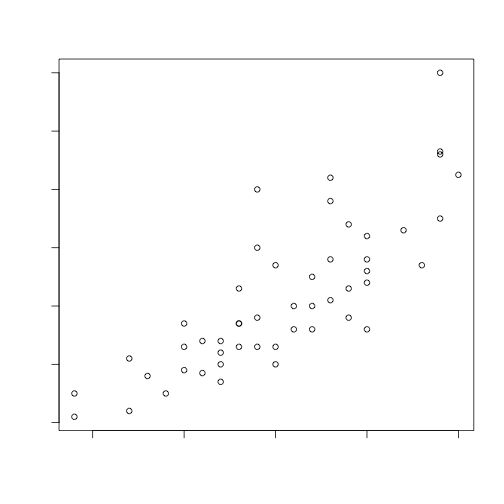
\includegraphics{Labo5_extension_Théorème_central_limite_nouveau_files/figure-beamer/unnamed-chunk-1-1.pdf}

\begin{Shaded}
\begin{Highlighting}[]
\NormalTok{?dnorm}
\end{Highlighting}
\end{Shaded}

Propriété:

\begin{enumerate}
\def\labelenumi{\arabic{enumi}.}
\item
\end{enumerate}

\begin{itemize}
\tightlist
\item
  L'intervalle d'un écart-type de part et d'autre de la moyenne contient
  68\% de la distribution
\item
  L'intervalle de deux écart-types de part et d'autre de la moyenne
  contient 95\% de la distribution
\item
  L'intervalle de trois écart-types de part et d'autre de la moyenne
  contient 99,7\% de la distribution
\end{itemize}

Aussi, nous avons trouvé qu'étant donné une valeur, nous trouvons la
proportion sous la courbe:

P(X \textless{} 2) P(x \textless{} 2) - P(X \textless{} -2) donne le
pourcentage de la distribution comprise entre -2 et 2.

\begin{Shaded}
\begin{Highlighting}[]
\KeywordTok{ggplot}\NormalTok{(}\DataTypeTok{data =} \KeywordTok{data.frame}\NormalTok{(}\DataTypeTok{x =} \KeywordTok{c}\NormalTok{(}\OperatorTok{-}\DecValTok{4}\NormalTok{, }\DecValTok{4}\NormalTok{)), }\KeywordTok{aes}\NormalTok{(x)) }\OperatorTok{+}
\StringTok{  }\KeywordTok{stat_function}\NormalTok{(}\DataTypeTok{fun =}\NormalTok{ dnorm, }\DataTypeTok{args =} \KeywordTok{list}\NormalTok{(}\DataTypeTok{mean =} \DecValTok{0}\NormalTok{, }\DataTypeTok{sd =} \DecValTok{1}\NormalTok{), }\DataTypeTok{color =} \StringTok{"red"}\NormalTok{) }\OperatorTok{+}
\StringTok{  }\KeywordTok{stat_function}\NormalTok{(}\DataTypeTok{fun =}\NormalTok{ dnorm, }\DataTypeTok{args =} \KeywordTok{list}\NormalTok{(}\DataTypeTok{mean =} \DecValTok{0}\NormalTok{, }\DataTypeTok{sd =} \DecValTok{1}\NormalTok{), }\DataTypeTok{color =} \StringTok{"blue"}\NormalTok{,}
                \DataTypeTok{geom =} \StringTok{"area"}\NormalTok{, }\DataTypeTok{fill =} \StringTok{"lightblue"}\NormalTok{, }\DataTypeTok{xlim =} \KeywordTok{c}\NormalTok{(}\OperatorTok{-}\DecValTok{1}\NormalTok{, }\DecValTok{1}\NormalTok{)) }\OperatorTok{+}
\StringTok{    }\KeywordTok{stat_function}\NormalTok{(}\DataTypeTok{fun =}\NormalTok{ dnorm, }\DataTypeTok{args =} \KeywordTok{list}\NormalTok{(}\DataTypeTok{mean =} \DecValTok{0}\NormalTok{, }\DataTypeTok{sd =} \DecValTok{1}\NormalTok{), }\DataTypeTok{color =} \StringTok{"green"}\NormalTok{,}
                \DataTypeTok{geom =} \StringTok{"area"}\NormalTok{, }\DataTypeTok{fill =} \StringTok{"green"}\NormalTok{, }\DataTypeTok{xlim =} \KeywordTok{c}\NormalTok{(}\OperatorTok{-}\DecValTok{2}\NormalTok{, }\DecValTok{2}\NormalTok{), }\DataTypeTok{alpha =} \FloatTok{0.2}\NormalTok{)  }
\end{Highlighting}
\end{Shaded}

\includegraphics{Labo5_extension_Théorème_central_limite_nouveau_files/figure-beamer/unnamed-chunk-2-1.pdf}

Il est préférable de partir de l'intervalle et de déterminer plus
précisément le nombre d'écart-type qui délimite l'intervalle.

Ainsi, quel intervalle contient 60\% de la distribution. Autrement dit,
comme la courbe est symétrique, on dira que 30\% de la distribution se
trouve entre la moyenne et la valeur recherchée. Donc que 20\% se trouve
au-delà. Autrement dit, pour trouver cet intervalle, il suffit de
trouver

\begin{Shaded}
\begin{Highlighting}[]
\KeywordTok{ggplot}\NormalTok{(}\DataTypeTok{data =} \KeywordTok{data.frame}\NormalTok{(}\DataTypeTok{x =} \KeywordTok{c}\NormalTok{(}\OperatorTok{-}\DecValTok{4}\NormalTok{, }\DecValTok{4}\NormalTok{)), }\KeywordTok{aes}\NormalTok{(x)) }\OperatorTok{+}
\StringTok{  }\KeywordTok{stat_function}\NormalTok{(}\DataTypeTok{fun =}\NormalTok{ dnorm, }\DataTypeTok{args =} \KeywordTok{list}\NormalTok{(}\DataTypeTok{mean =} \DecValTok{0}\NormalTok{, }\DataTypeTok{sd =} \DecValTok{1}\NormalTok{), }\DataTypeTok{color =} \StringTok{"red"}\NormalTok{) }\OperatorTok{+}
\StringTok{  }\KeywordTok{stat_function}\NormalTok{(}\DataTypeTok{fun =}\NormalTok{ dnorm, }\DataTypeTok{args =} \KeywordTok{list}\NormalTok{(}\DataTypeTok{mean =} \DecValTok{0}\NormalTok{, }\DataTypeTok{sd =} \DecValTok{1}\NormalTok{),}
                \DataTypeTok{geom =} \StringTok{"area"}\NormalTok{, }\DataTypeTok{fill =} \StringTok{"lightblue"}\NormalTok{, }\DataTypeTok{xlim =} \KeywordTok{c}\NormalTok{(}\OperatorTok{-}\DecValTok{4}\NormalTok{, }\OperatorTok{-}\DecValTok{2}\NormalTok{, }\DataTypeTok{alpha =} \FloatTok{0.2}\NormalTok{)) }\OperatorTok{+}
\StringTok{    }\KeywordTok{stat_function}\NormalTok{(}\DataTypeTok{fun =}\NormalTok{ dnorm, }\DataTypeTok{args =} \KeywordTok{list}\NormalTok{(}\DataTypeTok{mean =} \DecValTok{0}\NormalTok{, }\DataTypeTok{sd =} \DecValTok{1}\NormalTok{),}
                \DataTypeTok{geom =} \StringTok{"area"}\NormalTok{, }\DataTypeTok{fill =} \StringTok{"green"}\NormalTok{, }\DataTypeTok{xlim =} \KeywordTok{c}\NormalTok{(}\OperatorTok{-}\DecValTok{4}\NormalTok{, }\DecValTok{2}\NormalTok{), }\DataTypeTok{alpha =} \FloatTok{0.2}\NormalTok{)  }
\end{Highlighting}
\end{Shaded}

\includegraphics{Labo5_extension_Théorème_central_limite_nouveau_files/figure-beamer/unnamed-chunk-3-1.pdf}

Prob(distribution \textless{} v1) = 0.2 nous donne tout simplement la
valeur de 20 ième percentile de la distribution

Prob(distribution \textless{} v2) = 0.8 dit que 80\% de la distribution
est supérieure à cette valeur. Or, ces valeurs ont été calculées pour
nous par les statisticiens.

On peut le calculer assez facilement avec la fonction qnorm.

\begin{Shaded}
\begin{Highlighting}[]
\NormalTok{v1 <-}\StringTok{ }\KeywordTok{qnorm}\NormalTok{(}\FloatTok{0.2}\NormalTok{, }\DataTypeTok{mean =} \DecValTok{0}\NormalTok{, }\DataTypeTok{sd =} \DecValTok{1}\NormalTok{)}
\NormalTok{v1}
\end{Highlighting}
\end{Shaded}

\begin{verbatim}
## [1] -0.8416212
\end{verbatim}

\begin{Shaded}
\begin{Highlighting}[]
\NormalTok{v2 <-}\StringTok{ }\KeywordTok{qnorm}\NormalTok{(}\FloatTok{0.8}\NormalTok{, }\DataTypeTok{mean =} \DecValTok{0}\NormalTok{, }\DataTypeTok{sd =} \DecValTok{1}\NormalTok{)}
\NormalTok{v2}
\end{Highlighting}
\end{Shaded}

\begin{verbatim}
## [1] 0.8416212
\end{verbatim}

Ainsi, on trouve que l'intervalle en question est {[}-0,84; 0,84{]}.

A +- 0,84 écart-type de la moyenne, environ 60\% de la distribution s'y
trouve.

\end{frame}

\section{Théorème central limite - Règle de l'Approximation
Normale}\label{thuxe9oruxe8me-central-limite---ruxe8gle-de-lapproximation-normale}

\begin{frame}{Dégré de fiabilité de l'échantillon}

\begin{itemize}
\tightlist
\item
  Le but de l'échantillonnage aléatoire est d'éffectuer une inférence
  relative à la population sous-jacente.
\item
  On souhaite que la moyenne de l'échantillon - \(\bar{X}\) soit une
  estimation proche de la moyenne de la population - \(\mu\).
\item
  But: comprendre que les grands échantillons sont plus fiables que les
  petits échantillons
\item
  Deux façons d'étudier le degré d'approximation de \(\mu\) par
  \(\bar{X}\).
\end{itemize}

\begin{enumerate}
\def\labelenumi{\arabic{enumi}.}
\tightlist
\item
  A partir de formules mathématiques
\item
  A partir de la distribution d'échantillonnage
\end{enumerate}

\url{https://www.tqmp.org/Vignettes/vol16-2/v004/v004.pdf}

\end{frame}

\begin{frame}{Moments de la moyenne de l'échantillon}

\begin{itemize}
\item
  On démontre que :
\item
  \(E(\bar{X}) = \mu\) : la moyenne de l'échantillonnage \(\bar{X}\)
  coïncidera en moyenne avec l'objectif, ie. \(\bar{X}\) égalisera
  \(\mu\)
\item
  Erreur-type d'échantillon (standard error) =
  \(SE = \sigma_{\bar{X}} = \frac{\sigma}{\sqrt{n}}\), où \(\sigma\) est
  l'écart-type (standard deviation) dans la population
\item
  L'erreur-type de \(\bar{X}\) diminue quand la taille de l'échantillon
  aléatoire augmente.
\item
  Plus l'échantillon est grand, plus \(\bar{X}\) donne une estimation
  exacte de la moyenne de la population.
\item
  \textbf{NB}: Ne pas confondre:
\item
  écart-type (en anglais, standard deviation) et
\item
  erreur-type ou écart type d'échantillon (en anglais, standard error)
\end{itemize}

\end{frame}

\begin{frame}{Forme de la distribution d'échantillonnage}

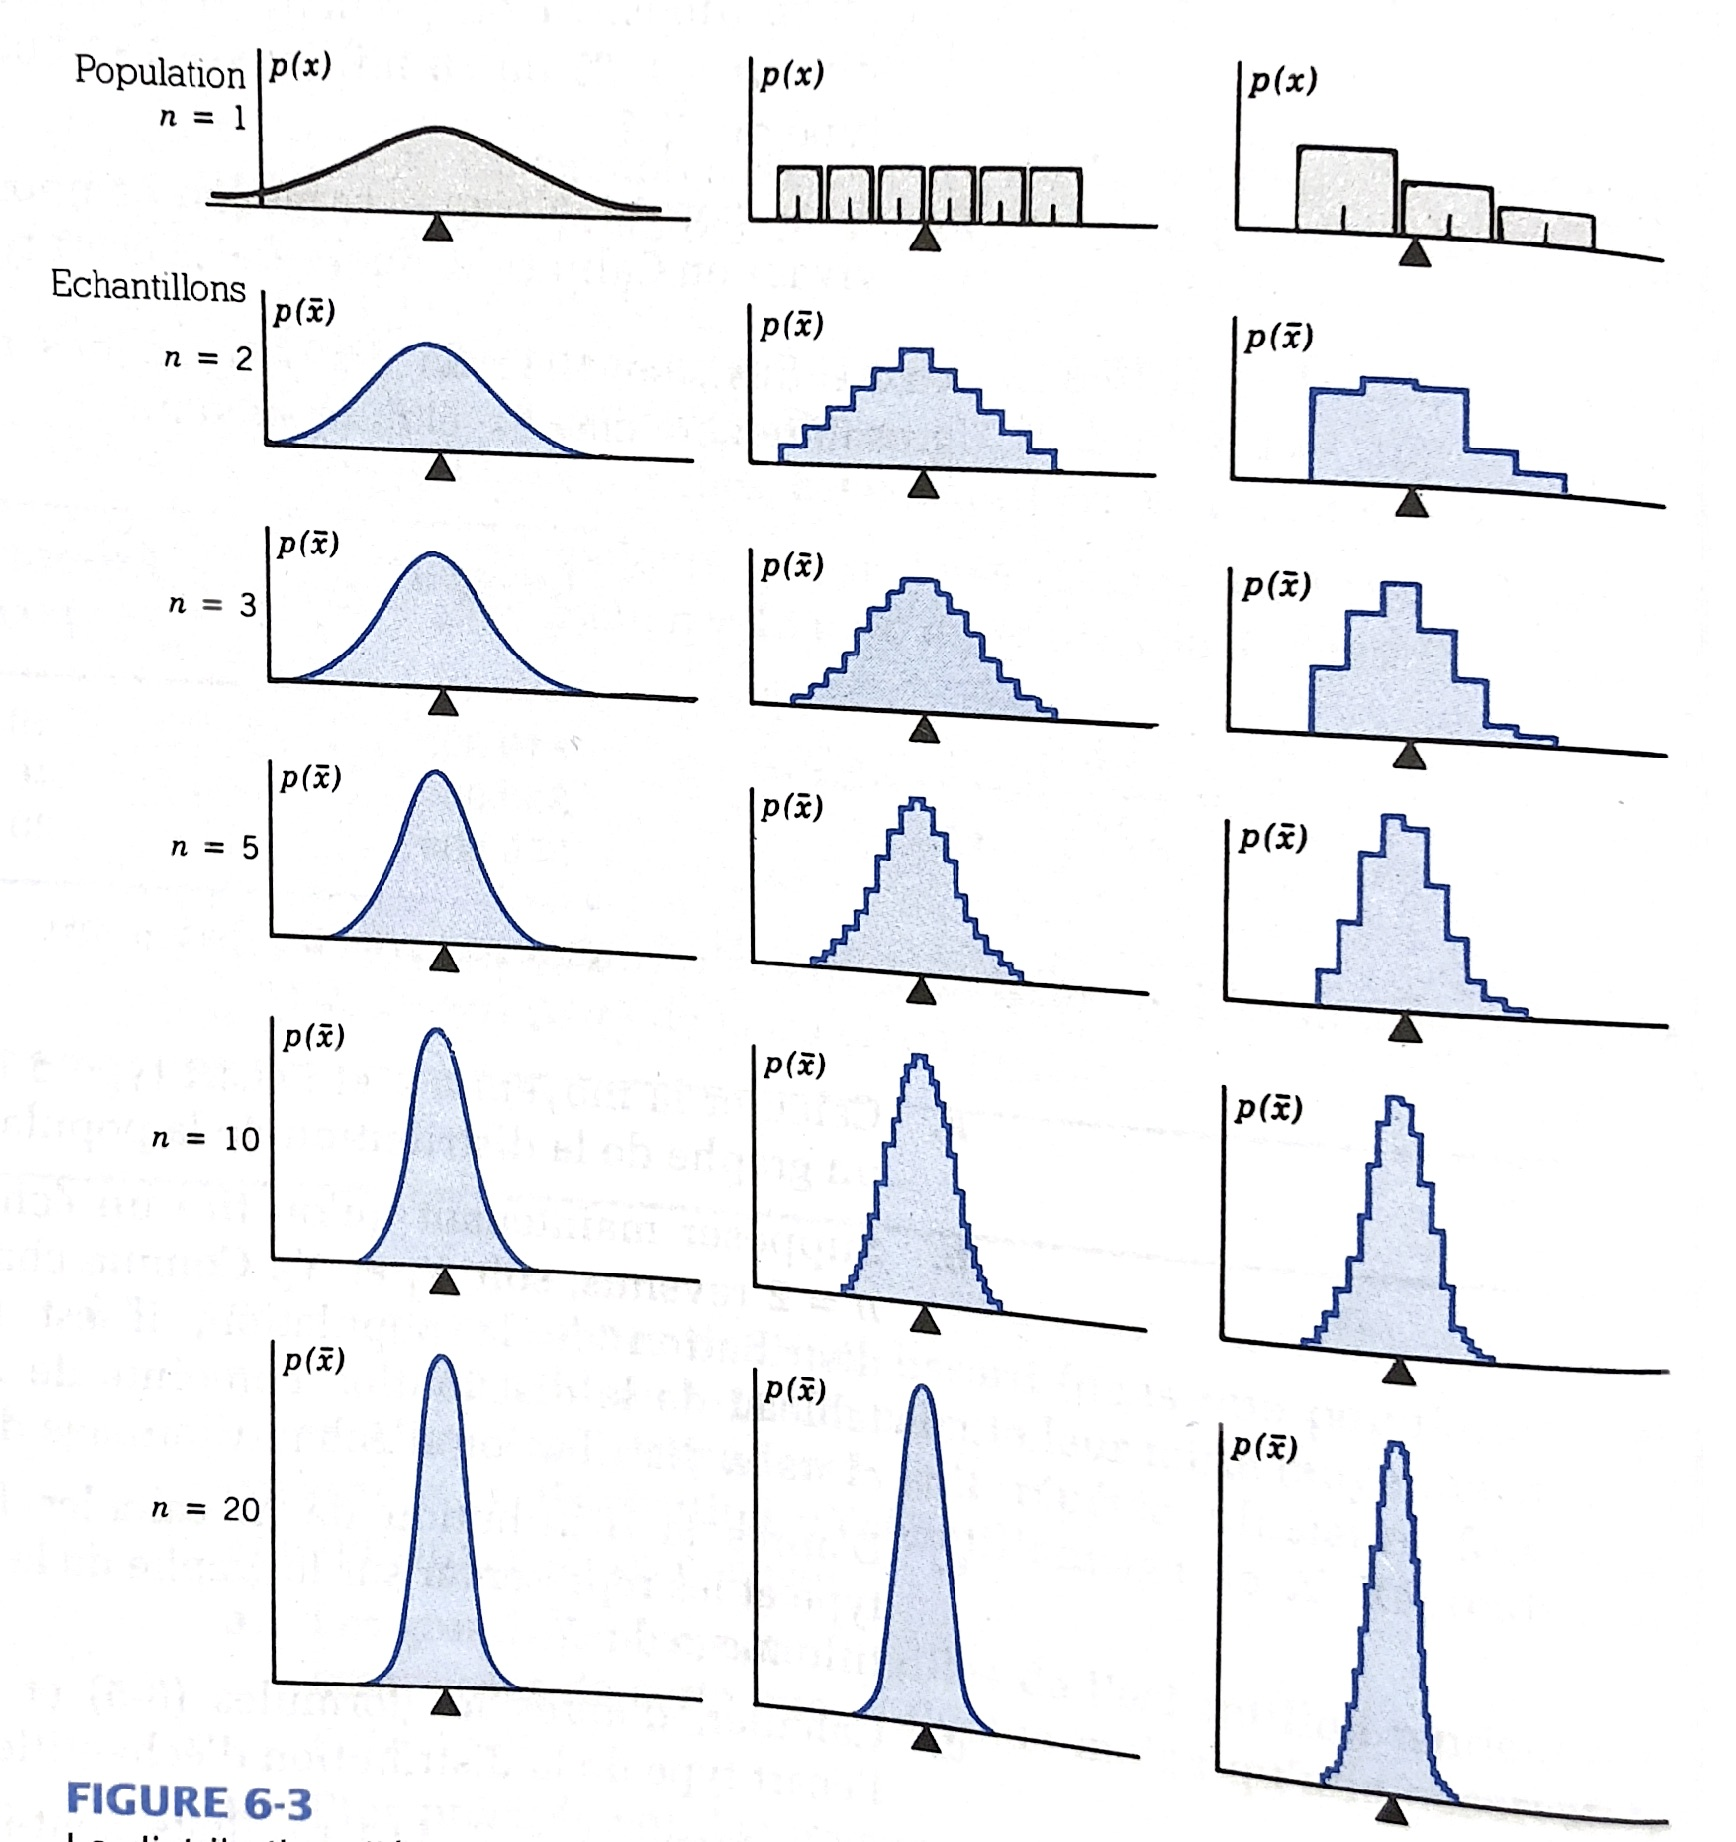
\includegraphics[width=0.7\linewidth]{distribution_echantillonnage}

\end{frame}

\begin{frame}{Théorème central limite (Règle de l'Approximation
Normale)}

Dans les échantillons aléatoires de taille n, la moyenne de
l'échantillon \(\bar{X}\) varie autour de la moyenne de la population
\(\mu\) avec une erreur-type égale à \(\frac{\sigma}{\sqrt{n}}\) (ou
\(\sigma\) est l'écart type de la population). Donc, quand n s'accroît,
la distribution d'échantillonnage de \(\bar{X}\) est de plus en plus
concentrée autour de son objectif \(\mu\). Elle devient de plus en plus
proche de la distribution normale (forme de cloche).

\end{frame}

\begin{frame}{Théorème central limite (Règle de l'Approximation
Normale)}

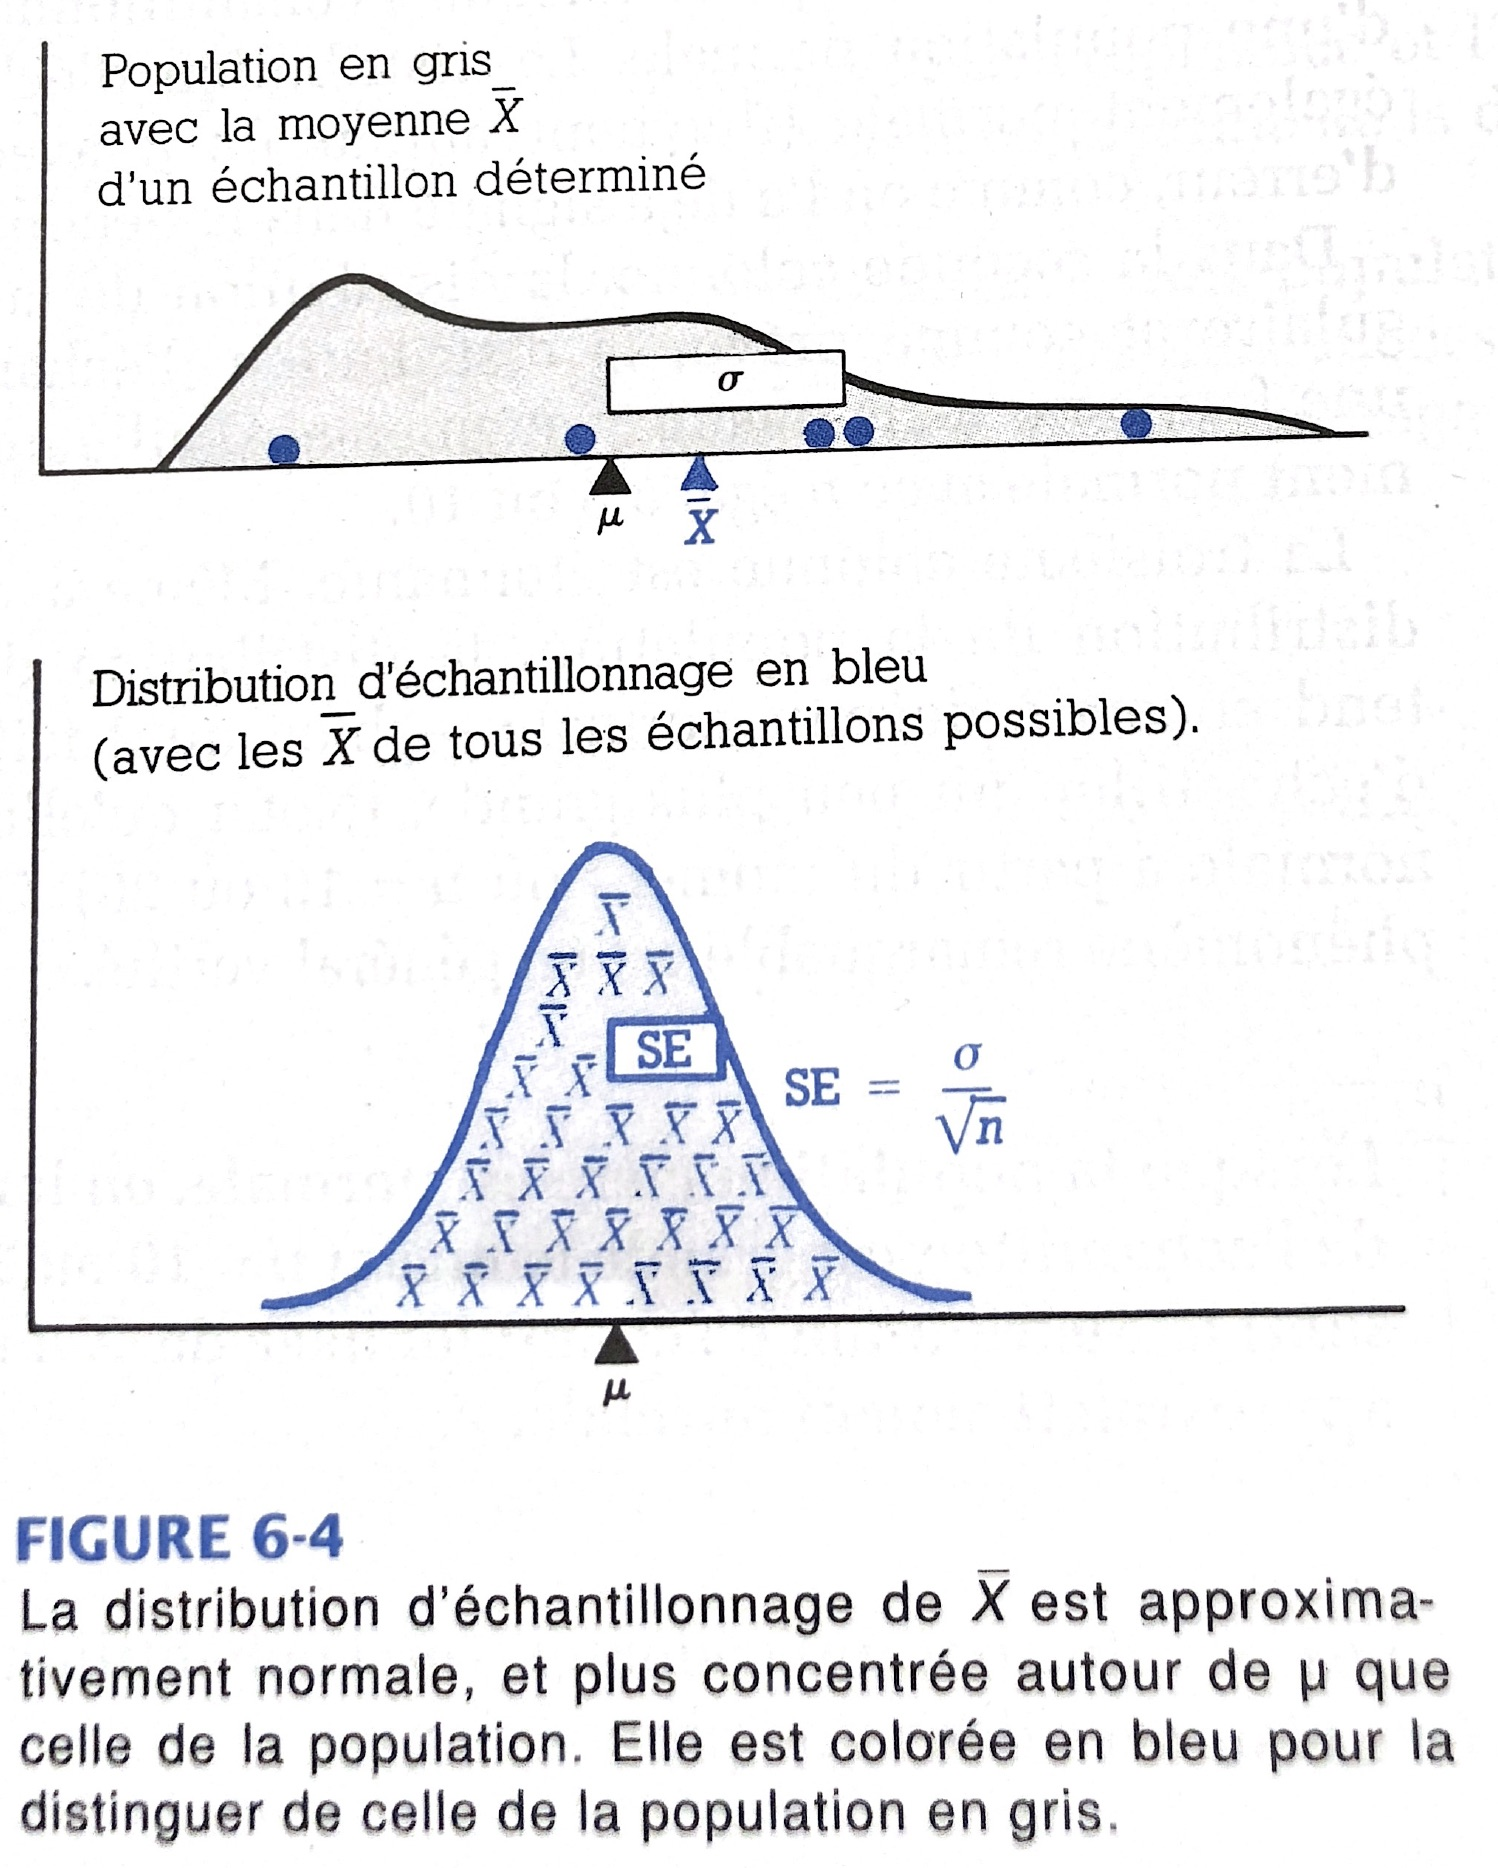
\includegraphics[width=0.7\linewidth]{tcl}

\end{frame}

\begin{frame}{Théorème central limite (Règle de l'Approximation
Normale)}

\begin{itemize}
\tightlist
\item
  Dire que la moyenne de l'échantillon \(\bar{X}\) varie autour de la
  moyenne de la population \(\mu\) avec une erreur type
  \(\sigma_{\bar{X}}\) égale à \(\frac{\sigma}{\sqrt{n}}\) revient à
  dire que la distribution \(\bar{X}\) suit une loi normale de moyenne
  \(\mu\) et d'écart type \(\frac{\sigma}{\sqrt{n}}\)
\item
  \(\bar{X}\) suit N(\(\mu\), \(\frac{\sigma}{\sqrt{n}}\))
\item
  Ou que (\(\frac{(\bar{X}-\mu)}{\frac{\sigma}{\sqrt{n}}}\)) suit une
  loi \textbf{normale dite centrée réduite} N(0,1)
\end{itemize}

\end{frame}

\begin{frame}[fragile]{Théorème central limite (Règle de l'Approximation
Normale) - Exemple}

Une population d'étudiants d'un grand campus du Middle-West a une taille
moyenne de \(\mu\) = 69 inches et un écart type \(\sigma\) = 3.22
inches. Si un échantillon aléatoire de n = 10 individus est prélevé,
quelle est la probabilité pour que la moyenne de l'échantillon
\(\bar{X}\) s'écarte de 2 inches de la moyenne de la population?

\begin{Shaded}
\begin{Highlighting}[]
\NormalTok{erreur_type <-}\StringTok{ }\FloatTok{3.22}\OperatorTok{/}\KeywordTok{sqrt}\NormalTok{(}\DecValTok{10}\NormalTok{)}
\NormalTok{erreur_type}
\end{Highlighting}
\end{Shaded}

\begin{verbatim}
## [1] 1.018253
\end{verbatim}

\begin{Shaded}
\begin{Highlighting}[]
\NormalTok{dis <-}\StringTok{ }

\NormalTok{distribution <-}
\StringTok{  }\KeywordTok{ggplot}\NormalTok{(}\DataTypeTok{data =} \KeywordTok{data.frame}\NormalTok{(}\DataTypeTok{x =} \KeywordTok{c}\NormalTok{(}\DecValTok{64}\NormalTok{, }\DecValTok{74}\NormalTok{)), }\KeywordTok{aes}\NormalTok{(x)) }\OperatorTok{+}
\StringTok{  }\KeywordTok{stat_function}\NormalTok{(}\DataTypeTok{fun =}\NormalTok{ dnorm, }\DataTypeTok{args =} \KeywordTok{list}\NormalTok{(}\DataTypeTok{mean =} \DecValTok{69}\NormalTok{, }\DataTypeTok{sd =}\NormalTok{ erreur_type), }\DataTypeTok{color =} \StringTok{"blue"}\NormalTok{) }\OperatorTok{+}
\StringTok{  }\KeywordTok{geom_vline}\NormalTok{(}\KeywordTok{aes}\NormalTok{(}\DataTypeTok{xintercept =} \DecValTok{71}\NormalTok{, }\DataTypeTok{color =} \StringTok{"red"}\NormalTok{)) }\OperatorTok{+}
\StringTok{  }\KeywordTok{geom_vline}\NormalTok{(}\KeywordTok{aes}\NormalTok{(}\DataTypeTok{xintercept =} \DecValTok{67}\NormalTok{, }\DataTypeTok{color =} \StringTok{"green"}\NormalTok{)) }\OperatorTok{+}
\StringTok{  }\KeywordTok{theme}\NormalTok{(}\DataTypeTok{legend.position =} \StringTok{"none"}\NormalTok{)}
\NormalTok{distribution}
\end{Highlighting}
\end{Shaded}

\includegraphics{Labo5_extension_Théorème_central_limite_nouveau_files/figure-beamer/unnamed-chunk-5-1.pdf}

\end{frame}

\begin{frame}{Théorème central limite (Règle de l'Approximation Normale)
- Exemple}

\begin{itemize}
\item
  \textbf{Réponse}:
\item
  Selon la Règle de l'Approximation Normale, \(\bar{X}\) est normalement
  distribuée avec:
\item
  Espérance = \(\mu\) = 69 et
\item
  Écart type d'échantillon = \(\sigma_{\bar{X}}\) =
  \(\frac{\sigma}{\sqrt{n}}\) = \(\frac{3.22}{\sqrt{10}}\) = 1.02
\item
  On cherche à déterminer la probabilité que \(\bar{X}\) s'écarte de 2
  inches de \(\mu\), c'est à dire qu'elle se trouve entre 67 et 71.
\item
  Aussi, calcule-t-on, d'abord la probabilité que \(\bar{X}\) soit
  supérieur à 71, en commençant par centrer et réduire:
  \[\text{Z = } \frac{\bar{X}-\mu}{\sigma_{\bar{X}}} = \frac{71 - 69}{1.02} = 1.96\]
\item
  Cela signifie que la valeur critique de 71 pour que la moyenne de
  l'échantillon est environ de 2 écarts-type au dessus de son espérance
  69.
\end{itemize}

\end{frame}

\begin{frame}{Théorème central limite (Règle de l'Approximation Normale)
- Exemple}

\begin{itemize}
\tightlist
\item
  D'après le tableau de la loi normale centrée réduite, on trouve que la
  probabilité que Z excède 1.96 est seulement de 0.025. C'est ce que
  montre la partie droite hachurée sur la figure (montrer la figure en
  classe).
\item
  En raison de la symétrie de la distribution normale, l'extrémité
  gauche a la même probabilité 0.025.
\item
  Ainsi, on peut déterminer la probabilité cherchée de la partie
  centrale : \[ Probabilité = 1.000 - 0.025 - 0.025 = 0.95\]
\item
  On conclut donc qu'il y a 95\% de chance pour que la moyenne de
  l'échantillon s'écarte de 2 inches de la moyenne de la population
\end{itemize}

\end{frame}

\begin{frame}{Théorème central limite (Règle de l'Approximation Normale)
- Question}

\begin{enumerate}
\def\labelenumi{\arabic{enumi}.}
\tightlist
\item
  Quelle est la probabilité que cette moyenne s'écarte de 1 inche de la
  moyenne de la population? Est-ce que cette probabilité va être plus
  grande ou plus pétite que la première?
\item
  Quelle est la probabilité que cette moyenne s'écarte de 3 inches de la
  moyenne de la population? Est-ce que cette probabilité va être plus
  grande ou plus pétite que la première?
\end{enumerate}

\end{frame}

\section{Application}\label{application}

\begin{frame}[fragile]{Introduction}

Nous allons travailler avec les données \texttt{bm\_results2012.txt} du
marathon de Boston de 2012. Le tableau ci-dessous présente les
informations contenues dans cette base de données.

\begin{longtable}[]{@{}ll@{}}
\toprule
Variables & Description\tabularnewline
\midrule
\endhead
V1 & Nom\tabularnewline
V2 & Sexe\tabularnewline
V3 & Age\tabularnewline
V4 & Division\tabularnewline
V5 & Pays\tabularnewline
V6 & Temps mis\tabularnewline
\bottomrule
\end{longtable}

\end{frame}

\begin{frame}[fragile]{Chargement de la base de données}

\begin{Shaded}
\begin{Highlighting}[]
\KeywordTok{rm}\NormalTok{(}\DataTypeTok{list =} \KeywordTok{ls}\NormalTok{())}
\NormalTok{marathon <-}\StringTok{ }\KeywordTok{read.csv}\NormalTok{(}\StringTok{"bm_results2012.txt"}\NormalTok{, }\DataTypeTok{header =} \OtherTok{FALSE}\NormalTok{, }\DataTypeTok{quote =} \StringTok{""}\NormalTok{)}
\end{Highlighting}
\end{Shaded}

\end{frame}

\begin{frame}[fragile]{Distribution de la variable V6}

\begin{itemize}
\item
  variable continue, on peut calculer les paramètres de tendance
  centrales et de dispersion
\item
  Position
\end{itemize}

\begin{Shaded}
\begin{Highlighting}[]
\CommentTok{# Moyenne}
\KeywordTok{mean}\NormalTok{(marathon}\OperatorTok{$}\NormalTok{V6)}
\end{Highlighting}
\end{Shaded}

\begin{verbatim}
## [1] 263.0493
\end{verbatim}

\begin{Shaded}
\begin{Highlighting}[]
\CommentTok{# Mediane}
\KeywordTok{median}\NormalTok{(marathon}\OperatorTok{$}\NormalTok{V6)}
\end{Highlighting}
\end{Shaded}

\begin{verbatim}
## [1] 255.82
\end{verbatim}

\begin{Shaded}
\begin{Highlighting}[]
\CommentTok{# Mode}
\end{Highlighting}
\end{Shaded}

On voit que le marathon de Boston est couru en moyenne à 263 minutes. La
moitié des coureurs sont arrivés avant 255.8 minutes alors que l'autre
moitié est arrivé après.

\begin{itemize}
\tightlist
\item
  Dispersion
\end{itemize}

\begin{Shaded}
\begin{Highlighting}[]
\CommentTok{# variance}
\KeywordTok{var}\NormalTok{(marathon}\OperatorTok{$}\NormalTok{V6)}
\end{Highlighting}
\end{Shaded}

\begin{verbatim}
## [1] 2502.422
\end{verbatim}

\begin{Shaded}
\begin{Highlighting}[]
\CommentTok{# Écart-type}
\KeywordTok{sd}\NormalTok{(marathon}\OperatorTok{$}\NormalTok{V6)}
\end{Highlighting}
\end{Shaded}

\begin{verbatim}
## [1] 50.02421
\end{verbatim}

La variance égale 2502 minutes au carré alors que l'écrat-type vaut 50
minutes. On sait que la variance n'est pas de la même unité de mesure
que la variable. C'est pourquoi on prend justement l'écart-type. En
soit, ces mesures ne nous apportent pas beaucoup d'information. C'est en
les comparant à une autre distribution qu'on peut tirer des conclusions.

On peut mieux présenter ces résultats en utilisant tydyverse

\begin{Shaded}
\begin{Highlighting}[]
\NormalTok{caract <-}\StringTok{ }
\StringTok{  }\NormalTok{marathon }\OperatorTok\StringTok{ }
\StringTok{  }\KeywordTok{summarise}\NormalTok{(}\DataTypeTok{moyenne =} \KeywordTok{mean}\NormalTok{(V6, }\DataTypeTok{na.rm =} \OtherTok{TRUE}\NormalTok{),}
            \DataTypeTok{ecarttype =} \KeywordTok{sd}\NormalTok{(V6, }\DataTypeTok{na.rm =} \OtherTok{TRUE}\NormalTok{),}
            \DataTypeTok{mediane =} \KeywordTok{median}\NormalTok{(V6, }\DataTypeTok{na.rm =} \OtherTok{TRUE}\NormalTok{),}
            \DataTypeTok{Q1 =} \KeywordTok{quantile}\NormalTok{(V6, }\DataTypeTok{prob =} \FloatTok{0.25}\NormalTok{),}
            \DataTypeTok{Q3 =} \KeywordTok{quantile}\NormalTok{(V6, }\DataTypeTok{prob =} \FloatTok{0.75}\NormalTok{),}
            \DataTypeTok{variance =} \KeywordTok{var}\NormalTok{(V6, }\DataTypeTok{na.rm =} \OtherTok{TRUE}\NormalTok{))}\OperatorTok\StringTok{ }
\StringTok{  }\KeywordTok{mutate}\NormalTok{(}\DataTypeTok{echantillon =} \KeywordTok{factor}\NormalTok{(}\StringTok{"Echantillon S1"}\NormalTok{))}

\NormalTok{caract}
\end{Highlighting}
\end{Shaded}

\begin{verbatim}
##    moyenne ecarttype mediane     Q1     Q3 variance    echantillon
## 1 263.0493  50.02421  255.82 228.78 290.73 2502.422 Echantillon S1
\end{verbatim}

\end{frame}

\begin{frame}[fragile]{Représentation graphique}

Il y a deux représentations qu'on fait d'une variable quantitative: -
l'histogramme - la boite à moustache

\begin{enumerate}
\def\labelenumi{\arabic{enumi}.}
\tightlist
\item
  Histogramme
\end{enumerate}

\begin{Shaded}
\begin{Highlighting}[]
\KeywordTok{library}\NormalTok{(tidyverse)}

\NormalTok{fig1 <-}\StringTok{ }
\StringTok{  }\KeywordTok{ggplot}\NormalTok{(marathon) }\OperatorTok{+}
\StringTok{  }\KeywordTok{geom_histogram}\NormalTok{(}\KeywordTok{aes}\NormalTok{(}\DataTypeTok{x =}\NormalTok{ V6), }\DataTypeTok{color=}\StringTok{"black"}\NormalTok{, }\DataTypeTok{fill=}\StringTok{"white"}\NormalTok{) }\OperatorTok{+}
\StringTok{  }\KeywordTok{geom_freqpoly}\NormalTok{(}\KeywordTok{aes}\NormalTok{(}\DataTypeTok{x =}\NormalTok{ V6), }\DataTypeTok{colour =} \StringTok{"blue"}\NormalTok{) }\OperatorTok{+}
\StringTok{  }\KeywordTok{stat_function}\NormalTok{(}\DataTypeTok{fun =}\NormalTok{ dnorm, }\DataTypeTok{args =} \KeywordTok{list}\NormalTok{(}\DataTypeTok{mean =} \KeywordTok{mean}\NormalTok{(marathon}\OperatorTok{$}\NormalTok{V6), }\DataTypeTok{sd =} \KeywordTok{sd}\NormalTok{(marathon}\OperatorTok{$}\NormalTok{V6)), }\DataTypeTok{colour =} \StringTok{"green"}\NormalTok{) }\OperatorTok{+}
\StringTok{  }\KeywordTok{geom_vline}\NormalTok{(}\KeywordTok{aes}\NormalTok{(}\DataTypeTok{xintercept =} \KeywordTok{mean}\NormalTok{(V6)), }\DataTypeTok{color =} \StringTok{"red"}\NormalTok{, }\DataTypeTok{linetype =} \StringTok{"dashed"}\NormalTok{) }\OperatorTok{+}
\StringTok{  }\KeywordTok{labs}\NormalTok{(}\DataTypeTok{title =} \StringTok{"Histogramme du Marathon de 2002"}\NormalTok{,}
       \DataTypeTok{x =} \StringTok{"Temps pour compléter le marathon"}\NormalTok{,}
       \DataTypeTok{y =} \StringTok{"Nombre de coureurs"}\NormalTok{)}
\end{Highlighting}
\end{Shaded}

\end{frame}

\begin{frame}[fragile]{Distribution de la variable V6}

\begin{Shaded}
\begin{Highlighting}[]
\NormalTok{fig1}
\end{Highlighting}
\end{Shaded}

\includegraphics[width=0.9\linewidth]{Labo5_extension_Théorème_central_limite_nouveau_files/figure-beamer/unnamed-chunk-11-1}

\end{frame}

\begin{frame}[fragile]{Boite à moustache}

\begin{Shaded}
\begin{Highlighting}[]
\KeywordTok{class}\NormalTok{(marathon}\OperatorTok{$}\NormalTok{V6)}
\end{Highlighting}
\end{Shaded}

\begin{verbatim}
## [1] "numeric"
\end{verbatim}

\begin{Shaded}
\begin{Highlighting}[]
\NormalTok{fig2 <-}\StringTok{ }
\StringTok{  }\KeywordTok{ggplot}\NormalTok{(marathon) }\OperatorTok{+}
\StringTok{  }\KeywordTok{geom_boxplot}\NormalTok{(}\KeywordTok{aes}\NormalTok{(}\DataTypeTok{y =}\NormalTok{ V6)) }\OperatorTok{+}
\StringTok{  }\KeywordTok{labs}\NormalTok{(}\DataTypeTok{title =} \StringTok{"Diagramme de quartile"}\NormalTok{,}
       \DataTypeTok{x =} \StringTok{""}\NormalTok{,}
       \DataTypeTok{y =} \StringTok{"Temps mis"}\NormalTok{)}
\end{Highlighting}
\end{Shaded}

\begin{Shaded}
\begin{Highlighting}[]
\NormalTok{fig2}
\end{Highlighting}
\end{Shaded}

\includegraphics{Labo5_extension_Théorème_central_limite_nouveau_files/figure-beamer/unnamed-chunk-13-1.pdf}

Dans la plupart des cas, nous ne disposons pas de l'information de la
population. Par exemple, pour estimer le revenu moyen de la population,
nous devons disposer d'un échantillon.

\end{frame}

\section{Échantillonnage aléatoire
simple}\label{uxe9chantillonnage-aluxe9atoire-simple}

\begin{frame}[fragile]{Échantillonnage aléatoire simple}

On appelle échantillonnage aléatoire simple celui où chaque individu de
la population \textbf{a la même chance d'être choisi} chaque fois que
l'on tire une observation.

\begin{itemize}
\tightlist
\item
  Maintenant, prenons un échantillon de cette population et analysons
  ses caractéristiques
\end{itemize}

\begin{Shaded}
\begin{Highlighting}[]
\KeywordTok{set.seed}\NormalTok{(}\DecValTok{430}\NormalTok{)}
\NormalTok{marathon_S1 <-}\StringTok{ }\KeywordTok{sample_n}\NormalTok{(marathon, }\DecValTok{40}\NormalTok{, }\DataTypeTok{replace =} \OtherTok{FALSE}\NormalTok{)}

\KeywordTok{head}\NormalTok{(marathon_S1)}
\end{Highlighting}
\end{Shaded}

\begin{verbatim}
##                    V1 V2 V3   V4  V5     V6
## 1    "Hellard Dwayne"  M 51 1196 USA 267.20
## 2       "Aron Narcis"  M 63  287 USA 278.40
## 3 "Owens Katherine H"  F 51  348 USA 272.72
## 4   "Takach Laura E."  F 28 4473 USA 380.85
## 5  "Frost Kathleen A"  F 46 1160 USA 301.33
## 6     "Minder Walter"  M 48 1667 SUI 274.08
\end{verbatim}

\end{frame}

\begin{frame}[fragile]{Échantillonnage aléatoire simple}

\begin{Shaded}
\begin{Highlighting}[]
\KeywordTok{ggplot}\NormalTok{(marathon_S1) }\OperatorTok{+}
\StringTok{  }\KeywordTok{geom_histogram}\NormalTok{(}\KeywordTok{aes}\NormalTok{(}\DataTypeTok{x =}\NormalTok{ V6)) }\OperatorTok{+}
\StringTok{  }\KeywordTok{labs}\NormalTok{(}\DataTypeTok{title =} \StringTok{"Histogramme du Marathon de 2012"}\NormalTok{,}
       \DataTypeTok{x =} \StringTok{"Temps pour compléter le marathon"}\NormalTok{,}
       \DataTypeTok{y =} \StringTok{"Nombre de coureurs"}\NormalTok{)}
\end{Highlighting}
\end{Shaded}

\includegraphics[width=0.6\linewidth,height=0.7\textheight]{Labo5_extension_Théorème_central_limite_nouveau_files/figure-beamer/unnamed-chunk-15-1}

\end{frame}

\begin{frame}[fragile]{Échantillonnage aléatoire simple}

\begin{Shaded}
\begin{Highlighting}[]
\NormalTok{caract_S1 <-}\StringTok{ }
\StringTok{  }\NormalTok{marathon_S1 }\OperatorTok\StringTok{ }
\StringTok{  }\KeywordTok{summarise}\NormalTok{(}\DataTypeTok{moyenne =} \KeywordTok{mean}\NormalTok{(V6, }\DataTypeTok{na.rm =} \OtherTok{TRUE}\NormalTok{),}
            \DataTypeTok{ecarttype =} \KeywordTok{sd}\NormalTok{(V6, }\DataTypeTok{na.rm =} \OtherTok{TRUE}\NormalTok{),}
            \DataTypeTok{mediane =} \KeywordTok{median}\NormalTok{(V6, }\DataTypeTok{na.rm =} \OtherTok{TRUE}\NormalTok{),}
            \DataTypeTok{Q1 =} \KeywordTok{quantile}\NormalTok{(V6, }\DataTypeTok{prob =} \FloatTok{0.25}\NormalTok{),}
            \DataTypeTok{Q3 =} \KeywordTok{quantile}\NormalTok{(V6, }\DataTypeTok{prob =} \FloatTok{0.75}\NormalTok{),}
            \DataTypeTok{variance =} \KeywordTok{var}\NormalTok{(V6, }\DataTypeTok{na.rm =} \OtherTok{TRUE}\NormalTok{))}\OperatorTok\StringTok{ }
\StringTok{  }\KeywordTok{mutate}\NormalTok{(}\DataTypeTok{echantillon =} \KeywordTok{factor}\NormalTok{(}\StringTok{"Echantillon S1"}\NormalTok{))}

\NormalTok{caract_S1}
\end{Highlighting}
\end{Shaded}

\begin{verbatim}
##    moyenne ecarttype mediane      Q1     Q3 variance    echantillon
## 1 268.5303  45.23583  263.25 237.465 284.04  2046.28 Echantillon S1
\end{verbatim}

\end{frame}

\begin{frame}[fragile]{Échantillonnage aléatoire simple - Comparaison de
la moyenne d'échantillon et la moyenne de population}

\begin{Shaded}
\begin{Highlighting}[]
\CommentTok{# Comparaison}
\NormalTok{caract_c <-}\StringTok{ }\KeywordTok{bind_rows}\NormalTok{(caract, caract_S1)}
\NormalTok{caract_c}
\end{Highlighting}
\end{Shaded}

\begin{verbatim}
##    moyenne ecarttype mediane      Q1     Q3 variance    echantillon
## 1 263.0493  50.02421  255.82 228.780 290.73 2502.422 Echantillon S1
## 2 268.5303  45.23583  263.25 237.465 284.04 2046.280 Echantillon S1
\end{verbatim}

\end{frame}

\begin{frame}[fragile]{Est-ce que cet échantillon est représentatif?}

\begin{Shaded}
\begin{Highlighting}[]
\KeywordTok{library}\NormalTok{(summarytools)}

\KeywordTok{freq}\NormalTok{(marathon}\OperatorTok{$}\NormalTok{V2)}
\end{Highlighting}
\end{Shaded}

\begin{verbatim}
## Frequencies  
## marathon$V2  
## Type: Factor  
## 
##                Freq   % Valid   % Valid Cum.   % Total   % Total Cum.
## ----------- ------- --------- -------------- --------- --------------
##           F    8959     41.59          41.59     41.59          41.59
##           M   12582     58.41         100.00     58.41         100.00
##        <NA>       0                               0.00         100.00
##       Total   21541    100.00         100.00    100.00         100.00
\end{verbatim}

\begin{Shaded}
\begin{Highlighting}[]
\KeywordTok{freq}\NormalTok{(marathon_S1}\OperatorTok{$}\NormalTok{V2)}
\end{Highlighting}
\end{Shaded}

\begin{verbatim}
## Frequencies  
## marathon_S1$V2  
## Type: Factor  
## 
##               Freq   % Valid   % Valid Cum.   % Total   % Total Cum.
## ----------- ------ --------- -------------- --------- --------------
##           F     17     42.50          42.50     42.50          42.50
##           M     23     57.50         100.00     57.50         100.00
##        <NA>      0                               0.00         100.00
##       Total     40    100.00         100.00    100.00         100.00
\end{verbatim}

\end{frame}

\section{Échantillonnage aléatoire simple - distribution
d'échantillonnage}\label{uxe9chantillonnage-aluxe9atoire-simple---distribution-duxe9chantillonnage}

\begin{frame}[fragile]{100 échantillons de taille 10}

\begin{Shaded}
\begin{Highlighting}[]
\KeywordTok{library}\NormalTok{(tidyverse)}
\end{Highlighting}
\end{Shaded}

\begin{itemize}
\tightlist
\item
  Ressource:
  \url{https://stackoverflow.com/questions/42676348/multiple-random-sampling-in-r}
\end{itemize}

\begin{Shaded}
\begin{Highlighting}[]
\KeywordTok{set.seed}\NormalTok{(}\DecValTok{123432}\NormalTok{)}
\NormalTok{marat_T10_R100 <-}\StringTok{ }\KeywordTok{bind_rows}\NormalTok{(}\KeywordTok{replicate}\NormalTok{(}\DecValTok{100}\NormalTok{, marathon }\OperatorTok\StringTok{ }\KeywordTok{sample_n}\NormalTok{(}\DecValTok{10}\NormalTok{, }\DataTypeTok{replace =} \OtherTok{FALSE}\NormalTok{), }\DataTypeTok{simplify =}\NormalTok{ F), }\DataTypeTok{.id =} \StringTok{"Obs"}\NormalTok{)}

\KeywordTok{glimpse}\NormalTok{(marat_T10_R100)}
\end{Highlighting}
\end{Shaded}

\begin{verbatim}
## Rows: 1,000
## Columns: 7
## $ Obs <chr> "1", "1", "1", "1", "1", "1", "1", "1", "1", "1", "2", "2", "2", "~
## $ V1  <fct> "Wild Lindsey", "Bellman Catherine S", "Lynch John", "Opel Jonatho~
## $ V2  <fct> F, F, M, M, F, M, M, M, M, F, M, F, M, F, M, F, M, M, M, F, M, M, ~
## $ V3  <int> 29, 56, 34, 36, 26, 25, 53, 48, 44, 36, 40, 38, 45, 32, 32, 46, 32~
## $ V4  <dbl> 189, 218, 2871, 330, 594, 49, 847, 238, 1919, 3360, 1943, 2642, 15~
## $ V5  <fct> USA, USA, USA, USA, USA, USA, USA, USA, USA, USA, USA, USA, CAN, U~
## $ V6  <dbl> 204.62, 301.40, 245.33, 178.10, 222.97, 157.22, 257.67, 208.78, 34~
\end{verbatim}

\end{frame}

\begin{frame}[fragile]{100 échantillons de taille 10}

\begin{Shaded}
\begin{Highlighting}[]
\NormalTok{caract_marat_T10_R100 <-}
\StringTok{  }\NormalTok{marat_T10_R100 }\OperatorTok\StringTok{ }
\StringTok{  }\KeywordTok{group_by}\NormalTok{(Obs) }\OperatorTok\StringTok{ }
\StringTok{  }\KeywordTok{summarise}\NormalTok{(}\DataTypeTok{moyenne =} \KeywordTok{mean}\NormalTok{(V6, }\DataTypeTok{na.rm =} \OtherTok{TRUE}\NormalTok{),}
            \DataTypeTok{ecarttype =} \KeywordTok{sd}\NormalTok{(V6, }\DataTypeTok{na.rm =} \OtherTok{TRUE}\NormalTok{)) }\OperatorTok\StringTok{ }
\StringTok{  }\KeywordTok{mutate}\NormalTok{(}\DataTypeTok{Taille =} \KeywordTok{factor}\NormalTok{(}\StringTok{"10"}\NormalTok{))}

\KeywordTok{glimpse}\NormalTok{(caract_marat_T10_R100)}
\end{Highlighting}
\end{Shaded}

\begin{verbatim}
## Rows: 100
## Columns: 4
## $ Obs       <chr> "1", "10", "100", "11", "12", "13", "14", "15", "16", "17", ~
## $ moyenne   <dbl> 241.597, 272.800, 263.271, 304.598, 244.785, 292.280, 247.78~
## $ ecarttype <dbl> 58.93145, 47.12677, 46.92948, 40.34323, 44.58382, 76.09095, ~
## $ Taille    <fct> 10, 10, 10, 10, 10, 10, 10, 10, 10, 10, 10, 10, 10, 10, 10, ~
\end{verbatim}

\end{frame}

\begin{frame}[fragile]{100 échantillons de taille 10 : Vérification du
théorème central limite}

\begin{Shaded}
\begin{Highlighting}[]
\NormalTok{esperance_moyenne <-}\StringTok{ }\KeywordTok{mean}\NormalTok{(caract_marat_T10_R100}\OperatorTok{$}\NormalTok{moyenne)}
\NormalTok{erreurtype <-}\StringTok{ }\KeywordTok{sd}\NormalTok{(caract_marat_T10_R100}\OperatorTok{$}\NormalTok{moyenne)}

\NormalTok{population_moyenne <-}\StringTok{ }\KeywordTok{mean}\NormalTok{(marathon}\OperatorTok{$}\NormalTok{V6)}
\NormalTok{erreurtype_calcule <-}\StringTok{ }\KeywordTok{sd}\NormalTok{(marathon}\OperatorTok{$}\NormalTok{V6)}\OperatorTok{/}\KeywordTok{sqrt}\NormalTok{(}\DecValTok{10}\NormalTok{)}

\NormalTok{tcl_T10 <-}\StringTok{ }\KeywordTok{bind_cols}\NormalTok{(}\DataTypeTok{e_m =}\NormalTok{ esperance_moyenne, }\DataTypeTok{mu =}\NormalTok{ population_moyenne, }\DataTypeTok{et =}\NormalTok{ erreurtype, }\DataTypeTok{etc =}\NormalTok{ erreurtype_calcule) }

\NormalTok{tcl_T10}
\end{Highlighting}
\end{Shaded}

\begin{verbatim}
## # A tibble: 1 x 4
##     e_m    mu    et   etc
##   <dbl> <dbl> <dbl> <dbl>
## 1  262.  263.  16.5  15.8
\end{verbatim}

\end{frame}

\begin{frame}[fragile]{100 échantillons de taille 10 - Représentation
graphique}

\begin{Shaded}
\begin{Highlighting}[]
\NormalTok{obslevel <-}\StringTok{ }\KeywordTok{c}\NormalTok{(}\KeywordTok{seq}\NormalTok{(}\DecValTok{1}\OperatorTok{:}\DecValTok{100}\NormalTok{))}

\NormalTok{fig_T10_}\DecValTok{1}\NormalTok{ <-}
\StringTok{  }\KeywordTok{ggplot}\NormalTok{(caract_marat_T10_R100) }\OperatorTok{+}
\StringTok{  }\KeywordTok{geom_point}\NormalTok{(}\KeywordTok{aes}\NormalTok{(}\DataTypeTok{x =}\NormalTok{ Obs, }\DataTypeTok{y =}\NormalTok{ moyenne)) }\OperatorTok{+}
\StringTok{  }\KeywordTok{geom_hline}\NormalTok{(}\KeywordTok{aes}\NormalTok{(}\DataTypeTok{yintercept =} \KeywordTok{mean}\NormalTok{(moyenne)), }\DataTypeTok{colour =} \StringTok{"red"}\NormalTok{) }\OperatorTok{+}
\StringTok{  }\KeywordTok{geom_hline}\NormalTok{(}\DataTypeTok{data =}\NormalTok{ marathon, }\KeywordTok{aes}\NormalTok{(}\DataTypeTok{yintercept =} \KeywordTok{mean}\NormalTok{(V6)), }\DataTypeTok{colour =} \StringTok{"green"}\NormalTok{) }\OperatorTok{+}
\StringTok{  }\KeywordTok{scale_x_discrete}\NormalTok{(}\DataTypeTok{limits =}\NormalTok{ obslevel) }\OperatorTok{+}
\StringTok{  }\KeywordTok{theme}\NormalTok{(}\DataTypeTok{axis.text.x =} \KeywordTok{element_text}\NormalTok{(}\DataTypeTok{angle =} \OperatorTok{-}\DecValTok{60}\NormalTok{, }\DataTypeTok{hjust =} \DecValTok{1}\NormalTok{, }\DataTypeTok{size =} \DecValTok{6}\NormalTok{))}
\end{Highlighting}
\end{Shaded}

\end{frame}

\begin{frame}[fragile]{100 Échantillons de taille 10 - Représentation
graphique}

\begin{Shaded}
\begin{Highlighting}[]
\NormalTok{fig_T10_}\DecValTok{2}\NormalTok{ <-}\StringTok{ }
\StringTok{  }\KeywordTok{ggplot}\NormalTok{(caract_marat_T10_R100) }\OperatorTok{+}
\StringTok{  }\KeywordTok{geom_histogram}\NormalTok{(}\KeywordTok{aes}\NormalTok{(}\DataTypeTok{x =}\NormalTok{ moyenne)) }\OperatorTok{+}
\StringTok{  }\KeywordTok{geom_vline}\NormalTok{(}\KeywordTok{aes}\NormalTok{(}\DataTypeTok{xintercept =} \KeywordTok{mean}\NormalTok{(moyenne)), }\DataTypeTok{colour =} \StringTok{"red"}\NormalTok{) }\OperatorTok{+}
\StringTok{  }\KeywordTok{geom_vline}\NormalTok{(}\DataTypeTok{data =}\NormalTok{ marathon, }\KeywordTok{aes}\NormalTok{(}\DataTypeTok{xintercept =} \KeywordTok{mean}\NormalTok{(V6)), }\DataTypeTok{color =} \StringTok{"green"}\NormalTok{)}
\end{Highlighting}
\end{Shaded}

\end{frame}

\begin{frame}[fragile]{100 Échantillons de taille 10 - Représentation
graphique}

\begin{Shaded}
\begin{Highlighting}[]
\KeywordTok{library}\NormalTok{(ggpubr)}

\KeywordTok{ggarrange}\NormalTok{(fig_T10_}\DecValTok{1}\NormalTok{, fig_T10_}\DecValTok{2}\NormalTok{, }\DataTypeTok{ncol =} \DecValTok{2}\NormalTok{)}
\end{Highlighting}
\end{Shaded}

\includegraphics[width=0.9\linewidth,height=0.7\textheight]{Labo5_extension_Théorème_central_limite_nouveau_files/figure-beamer/unnamed-chunk-25-1}

\end{frame}

\begin{frame}[fragile]{100 échantillons de taille 30}

\begin{Shaded}
\begin{Highlighting}[]
\KeywordTok{set.seed}\NormalTok{(}\DecValTok{1234}\NormalTok{)}
\NormalTok{marat_T30_R100 <-}\StringTok{ }\KeywordTok{bind_rows}\NormalTok{(}\KeywordTok{replicate}\NormalTok{(}\DecValTok{100}\NormalTok{, marathon }\OperatorTok\StringTok{ }\KeywordTok{sample_n}\NormalTok{(}\DecValTok{30}\NormalTok{, }\DataTypeTok{replace =} \OtherTok{FALSE}\NormalTok{), }\DataTypeTok{simplify =}\NormalTok{ F), }\DataTypeTok{.id =} \StringTok{"Obs"}\NormalTok{)}

\NormalTok{caract_marat_T30_R100 <-}
\StringTok{  }\NormalTok{marat_T30_R100 }\OperatorTok\StringTok{ }
\StringTok{  }\KeywordTok{group_by}\NormalTok{(Obs) }\OperatorTok\StringTok{ }
\StringTok{  }\KeywordTok{summarise}\NormalTok{(}\DataTypeTok{moyenne =} \KeywordTok{mean}\NormalTok{(V6, }\DataTypeTok{na.rm =} \OtherTok{TRUE}\NormalTok{),}
            \DataTypeTok{ecarttype =} \KeywordTok{sd}\NormalTok{(V6, }\DataTypeTok{na.rm =} \OtherTok{TRUE}\NormalTok{)) }\OperatorTok\StringTok{ }
\StringTok{  }\KeywordTok{mutate}\NormalTok{(}\DataTypeTok{Taille =} \KeywordTok{factor}\NormalTok{(}\StringTok{"30"}\NormalTok{))}

\KeywordTok{head}\NormalTok{(caract_marat_T30_R100)}
\end{Highlighting}
\end{Shaded}

\begin{verbatim}
## # A tibble: 6 x 4
##   Obs   moyenne ecarttype Taille
##   <chr>   <dbl>     <dbl> <fct> 
## 1 1        260.      54.4 30    
## 2 10       259.      45.6 30    
## 3 100      268.      56.8 30    
## 4 11       246.      44.1 30    
## 5 12       272.      60.9 30    
## 6 13       268.      49.1 30
\end{verbatim}

\end{frame}

\begin{frame}[fragile]{100 échantillons de taille 30 : Vérification du
théorème central limite}

\begin{Shaded}
\begin{Highlighting}[]
\NormalTok{esperance_moyenne <-}\StringTok{ }\KeywordTok{mean}\NormalTok{(caract_marat_T30_R100}\OperatorTok{$}\NormalTok{moyenne)}
\NormalTok{erreurtype <-}\StringTok{ }\KeywordTok{sd}\NormalTok{(caract_marat_T30_R100}\OperatorTok{$}\NormalTok{moyenne)}

\NormalTok{population_moyenne <-}\StringTok{ }\KeywordTok{mean}\NormalTok{(marathon}\OperatorTok{$}\NormalTok{V6)}
\NormalTok{erreurtype_calcule <-}\StringTok{ }\KeywordTok{sd}\NormalTok{(marathon}\OperatorTok{$}\NormalTok{V6)}\OperatorTok{/}\KeywordTok{sqrt}\NormalTok{(}\DecValTok{30}\NormalTok{)}

\NormalTok{tcl_T30 <-}\StringTok{ }\KeywordTok{bind_cols}\NormalTok{(}\DataTypeTok{e_m =}\NormalTok{ esperance_moyenne, }\DataTypeTok{mu =}\NormalTok{ population_moyenne, }\DataTypeTok{et =}\NormalTok{ erreurtype, }\DataTypeTok{etc =}\NormalTok{ erreurtype_calcule) }

\NormalTok{tcl_T30}
\end{Highlighting}
\end{Shaded}

\begin{verbatim}
## # A tibble: 1 x 4
##     e_m    mu    et   etc
##   <dbl> <dbl> <dbl> <dbl>
## 1  264.  263.  8.95  9.13
\end{verbatim}

\end{frame}

\begin{frame}[fragile]{100 échantillons de taille 30}

\begin{Shaded}
\begin{Highlighting}[]
\CommentTok{#obslevel <- c(seq(1:100))}

\NormalTok{fig_T30_}\DecValTok{1}\NormalTok{ <-}\StringTok{ }
\StringTok{  }\KeywordTok{ggplot}\NormalTok{(caract_marat_T30_R100) }\OperatorTok{+}
\StringTok{  }\KeywordTok{geom_point}\NormalTok{(}\KeywordTok{aes}\NormalTok{(}\DataTypeTok{x =}\NormalTok{ Obs, }\DataTypeTok{y =}\NormalTok{ moyenne)) }\OperatorTok{+}
\StringTok{  }\KeywordTok{geom_hline}\NormalTok{(}\KeywordTok{aes}\NormalTok{(}\DataTypeTok{yintercept =} \KeywordTok{mean}\NormalTok{(moyenne)), }\DataTypeTok{colour =} \StringTok{"red"}\NormalTok{) }\OperatorTok{+}
\StringTok{  }\KeywordTok{geom_hline}\NormalTok{(}\DataTypeTok{data =}\NormalTok{ marathon, }\KeywordTok{aes}\NormalTok{(}\DataTypeTok{yintercept =} \KeywordTok{mean}\NormalTok{(V6)), }\DataTypeTok{colour =} \StringTok{"green"}\NormalTok{) }\OperatorTok{+}
\StringTok{  }\KeywordTok{scale_x_discrete}\NormalTok{(}\DataTypeTok{limits =}\NormalTok{ obslevel) }\OperatorTok{+}
\StringTok{  }\KeywordTok{theme}\NormalTok{(}\DataTypeTok{axis.text.x =} \KeywordTok{element_text}\NormalTok{(}\DataTypeTok{angle =} \OperatorTok{-}\DecValTok{60}\NormalTok{, }\DataTypeTok{hjust =} \DecValTok{1}\NormalTok{, }\DataTypeTok{size =} \DecValTok{6}\NormalTok{))}
\end{Highlighting}
\end{Shaded}

\end{frame}

\begin{frame}[fragile]{100 Échantillons de taille 30 - Représentation
graphique}

\begin{Shaded}
\begin{Highlighting}[]
\NormalTok{fig_T30_}\DecValTok{2}\NormalTok{ <-}\StringTok{ }
\StringTok{  }\KeywordTok{ggplot}\NormalTok{(caract_marat_T30_R100) }\OperatorTok{+}
\StringTok{  }\KeywordTok{geom_histogram}\NormalTok{(}\KeywordTok{aes}\NormalTok{(}\DataTypeTok{x =}\NormalTok{ moyenne)) }\OperatorTok{+}
\StringTok{  }\KeywordTok{geom_vline}\NormalTok{(}\KeywordTok{aes}\NormalTok{(}\DataTypeTok{xintercept =} \KeywordTok{mean}\NormalTok{(moyenne)), }\DataTypeTok{colour =} \StringTok{"red"}\NormalTok{) }\OperatorTok{+}
\StringTok{  }\KeywordTok{geom_vline}\NormalTok{(}\DataTypeTok{data =}\NormalTok{ marathon, }\KeywordTok{aes}\NormalTok{(}\DataTypeTok{xintercept =} \KeywordTok{mean}\NormalTok{(V6)), }\DataTypeTok{color =} \StringTok{"green"}\NormalTok{)}
\end{Highlighting}
\end{Shaded}

\end{frame}

\begin{frame}[fragile]{100 Échantillons de taille 30 - Représentation
graphique}

\begin{Shaded}
\begin{Highlighting}[]
\KeywordTok{ggarrange}\NormalTok{(fig_T30_}\DecValTok{1}\NormalTok{, fig_T30_}\DecValTok{2}\NormalTok{, }\DataTypeTok{ncol =} \DecValTok{2}\NormalTok{)}
\end{Highlighting}
\end{Shaded}

\includegraphics[width=0.9\linewidth,height=0.7\textheight]{Labo5_extension_Théorème_central_limite_nouveau_files/figure-beamer/unnamed-chunk-30-1}

\end{frame}

\begin{frame}[fragile]{100 échantillons de tailles 50}

\begin{Shaded}
\begin{Highlighting}[]
\KeywordTok{set.seed}\NormalTok{(}\DecValTok{12302}\NormalTok{)}
\NormalTok{marat_T50_R100 <-}\StringTok{ }\KeywordTok{bind_rows}\NormalTok{(}\KeywordTok{replicate}\NormalTok{(}\DecValTok{100}\NormalTok{, marathon }\OperatorTok\StringTok{ }\KeywordTok{sample_n}\NormalTok{(}\DecValTok{50}\NormalTok{, }\DataTypeTok{replace =} \OtherTok{FALSE}\NormalTok{), }\DataTypeTok{simplify =}\NormalTok{ F), }\DataTypeTok{.id =} \StringTok{"Obs"}\NormalTok{)}

\NormalTok{caract_marat_T50_R100 <-}
\StringTok{  }\NormalTok{marat_T50_R100 }\OperatorTok\StringTok{ }
\StringTok{  }\KeywordTok{group_by}\NormalTok{(Obs) }\OperatorTok\StringTok{ }
\StringTok{  }\KeywordTok{summarise}\NormalTok{(}\DataTypeTok{moyenne =} \KeywordTok{mean}\NormalTok{(V6, }\DataTypeTok{na.rm =} \OtherTok{TRUE}\NormalTok{),}
            \DataTypeTok{ecarttype =} \KeywordTok{sd}\NormalTok{(V6, }\DataTypeTok{na.rm =} \OtherTok{TRUE}\NormalTok{))}\OperatorTok\StringTok{ }
\StringTok{  }\KeywordTok{mutate}\NormalTok{(}\DataTypeTok{Taille =} \KeywordTok{factor}\NormalTok{(}\StringTok{"50"}\NormalTok{)) }

\KeywordTok{glimpse}\NormalTok{(caract_marat_T50_R100)}
\end{Highlighting}
\end{Shaded}

\begin{verbatim}
## Rows: 100
## Columns: 4
## $ Obs       <chr> "1", "10", "100", "11", "12", "13", "14", "15", "16", "17", ~
## $ moyenne   <dbl> 264.9438, 258.6650, 259.2164, 261.0740, 279.7738, 264.2202, ~
## $ ecarttype <dbl> 46.45658, 49.27246, 59.92799, 38.43878, 50.41155, 42.75819, ~
## $ Taille    <fct> 50, 50, 50, 50, 50, 50, 50, 50, 50, 50, 50, 50, 50, 50, 50, ~
\end{verbatim}

\end{frame}

\begin{frame}[fragile]{100 échantillons de taille 50 : Vérification du
théorème central limite}

\begin{Shaded}
\begin{Highlighting}[]
\NormalTok{esperance_moyenne <-}\StringTok{ }\KeywordTok{mean}\NormalTok{(caract_marat_T50_R100}\OperatorTok{$}\NormalTok{moyenne)}
\NormalTok{erreurtype <-}\StringTok{ }\KeywordTok{sd}\NormalTok{(caract_marat_T50_R100}\OperatorTok{$}\NormalTok{moyenne)}

\NormalTok{population_moyenne <-}\StringTok{ }\KeywordTok{mean}\NormalTok{(marathon}\OperatorTok{$}\NormalTok{V6)}
\NormalTok{erreurtype_calcule <-}\StringTok{ }\KeywordTok{sd}\NormalTok{(marathon}\OperatorTok{$}\NormalTok{V6)}\OperatorTok{/}\KeywordTok{sqrt}\NormalTok{(}\DecValTok{50}\NormalTok{)}

\NormalTok{tcl_T50 <-}\StringTok{ }\KeywordTok{bind_cols}\NormalTok{(}\DataTypeTok{e_m =}\NormalTok{ esperance_moyenne, }\DataTypeTok{mu =}\NormalTok{ population_moyenne, }\DataTypeTok{et =}\NormalTok{ erreurtype, }\DataTypeTok{etc =}\NormalTok{ erreurtype_calcule) }

\NormalTok{tcl_T50}
\end{Highlighting}
\end{Shaded}

\begin{verbatim}
## # A tibble: 1 x 4
##     e_m    mu    et   etc
##   <dbl> <dbl> <dbl> <dbl>
## 1  263.  263.  7.12  7.07
\end{verbatim}

\end{frame}

\begin{frame}[fragile]{100 échantillons de taille 50}

\begin{Shaded}
\begin{Highlighting}[]
\KeywordTok{ggplot}\NormalTok{(caract_marat_T50_R100) }\OperatorTok{+}
\StringTok{  }\KeywordTok{geom_histogram}\NormalTok{(}\KeywordTok{aes}\NormalTok{(}\DataTypeTok{x =}\NormalTok{ moyenne)) }\OperatorTok{+}
\StringTok{  }\KeywordTok{geom_point}\NormalTok{(}\KeywordTok{aes}\NormalTok{(}\DataTypeTok{x =}\NormalTok{ moyenne, }\DataTypeTok{y =}\NormalTok{ Obs)) }\OperatorTok{+}
\StringTok{  }\KeywordTok{geom_vline}\NormalTok{(}\KeywordTok{aes}\NormalTok{(}\DataTypeTok{xintercept =} \KeywordTok{mean}\NormalTok{(moyenne)), }\DataTypeTok{color =} \StringTok{"red"}\NormalTok{, }\DataTypeTok{size =} \FloatTok{0.1}\NormalTok{) }\OperatorTok{+}
\StringTok{  }\KeywordTok{geom_vline}\NormalTok{(}\DataTypeTok{data =}\NormalTok{ marathon, }\KeywordTok{aes}\NormalTok{(}\DataTypeTok{xintercept =} \KeywordTok{mean}\NormalTok{(V6)), }\DataTypeTok{color =} \StringTok{"green"}\NormalTok{, }\DataTypeTok{size =} \FloatTok{0.1}\NormalTok{)}
\end{Highlighting}
\end{Shaded}

\includegraphics[width=0.5\linewidth,height=0.7\textheight]{Labo5_extension_Théorème_central_limite_nouveau_files/figure-beamer/unnamed-chunk-33-1}

\end{frame}

\begin{frame}[fragile]{Comparaison de plusieurs distributions
d'échantillonnage}

\begin{Shaded}
\begin{Highlighting}[]
\NormalTok{fig_comp <-}\StringTok{ }
\StringTok{  }\KeywordTok{ggplot}\NormalTok{() }\OperatorTok{+}
\StringTok{  }\KeywordTok{geom_density}\NormalTok{(}\DataTypeTok{data =}\NormalTok{ caract_marat_T10_R100, }\KeywordTok{aes}\NormalTok{(}\DataTypeTok{x =}\NormalTok{ moyenne), }\DataTypeTok{colour =} \StringTok{"yellow"}\NormalTok{, }\DataTypeTok{fill =} \StringTok{"yellow"}\NormalTok{) }\OperatorTok{+}
\StringTok{  }\KeywordTok{geom_density}\NormalTok{(}\DataTypeTok{data =}\NormalTok{ caract_marat_T30_R100, }\KeywordTok{aes}\NormalTok{(}\DataTypeTok{x =}\NormalTok{ moyenne), }\DataTypeTok{colour =} \StringTok{"green"}\NormalTok{) }\OperatorTok{+}
\StringTok{  }\KeywordTok{geom_density}\NormalTok{(}\DataTypeTok{data =}\NormalTok{ caract_marat_T50_R100, }\KeywordTok{aes}\NormalTok{(}\DataTypeTok{x =}\NormalTok{ moyenne), }\DataTypeTok{colour =} \StringTok{"purple"}\NormalTok{) }\OperatorTok{+}
\StringTok{  }\KeywordTok{geom_density}\NormalTok{(}\DataTypeTok{data =}\NormalTok{ marathon, }\KeywordTok{aes}\NormalTok{(}\DataTypeTok{x =}\NormalTok{ V6), }\DataTypeTok{colour =} \StringTok{"red"}\NormalTok{) }\OperatorTok{+}
\StringTok{  }\KeywordTok{geom_vline}\NormalTok{(}\DataTypeTok{data =}\NormalTok{ marathon, }\KeywordTok{aes}\NormalTok{(}\DataTypeTok{xintercept =} \KeywordTok{mean}\NormalTok{(V6)), }\DataTypeTok{color =} \StringTok{"black"}\NormalTok{)}
\end{Highlighting}
\end{Shaded}

\end{frame}

\begin{frame}[fragile]{Comparaison de plusieurs distributions
d'échantillonnage}

\begin{Shaded}
\begin{Highlighting}[]
\NormalTok{fig_comp }
\end{Highlighting}
\end{Shaded}

\includegraphics{Labo5_extension_Théorème_central_limite_nouveau_files/figure-beamer/unnamed-chunk-35-1.pdf}

\end{frame}

\begin{frame}[fragile]{Fonction}

Nous avons sélectionné plusieurs échantillons en répliquant la meême
formule plusieurs fois. Essayons de voir si nous pouvons faire la meême
chose en utilisant les fonctions.

\begin{Shaded}
\begin{Highlighting}[]
\NormalTok{echantillon <-}\StringTok{ }\ControlFlowTok{function}\NormalTok{(k, donnee, n)\{}
  \KeywordTok{bind_rows}\NormalTok{(}\KeywordTok{replicate}\NormalTok{(k, donnee }\OperatorTok\StringTok{ }\KeywordTok{sample_n}\NormalTok{(n, }\DataTypeTok{replace =} \OtherTok{FALSE}\NormalTok{), }\DataTypeTok{simplify =}\NormalTok{ F), }\DataTypeTok{.id =} \StringTok{"Obs"}\NormalTok{)}

\NormalTok{\}}

\NormalTok{echantillon_t30_i100 <-}\StringTok{ }\KeywordTok{echantillon}\NormalTok{(}\DecValTok{100}\NormalTok{, marathon, }\DecValTok{30}\NormalTok{)}

\NormalTok{ech <-}\StringTok{ }\KeywordTok{c}\NormalTok{(}\StringTok{"taille5"}\NormalTok{, }\StringTok{"taille6"}\NormalTok{)}
\NormalTok{samp_k <-}\StringTok{ }\KeywordTok{vector}\NormalTok{(}\StringTok{"list"}\NormalTok{, }\DataTypeTok{length  =} \DecValTok{2}\NormalTok{)       }
\KeywordTok{names}\NormalTok{(samp_k) <-}\StringTok{ }\KeywordTok{names}\NormalTok{(ech)}
\ControlFlowTok{for}\NormalTok{ (i }\ControlFlowTok{in} \DecValTok{5}\OperatorTok{:}\DecValTok{6}\NormalTok{) \{}
\NormalTok{ samp_k[[i]] <-}\StringTok{ }\KeywordTok{echantillon}\NormalTok{(}\DecValTok{100}\NormalTok{, marathon, i)}
\NormalTok{  \}}


\CommentTok{#samp <- matrix(NA, nrow = length(echantillon), ncol = 7)}
\CommentTok{#names(samp) <- names(marathon)}
\CommentTok{#for (i in 5:6) \{}
\CommentTok{# samp[i, ] <- echantillon(100, marathon, i)}
\CommentTok{#  \}}
\end{Highlighting}
\end{Shaded}

\end{frame}

\section{Intervalle de confiance}\label{intervalle-de-confiance}

\begin{frame}[fragile]{Intervalle de confiance}

\begin{Shaded}
\begin{Highlighting}[]
\NormalTok{caract_marat_T30_R100 <-}
\StringTok{  }\NormalTok{caract_marat_T30_R100 }\OperatorTok\StringTok{ }
\StringTok{  }\KeywordTok{mutate}\NormalTok{(}\DataTypeTok{erreurtype =} \KeywordTok{sd}\NormalTok{(marathon}\OperatorTok{$}\NormalTok{V6)}\OperatorTok{/}\KeywordTok{sqrt}\NormalTok{(}\DecValTok{30}\NormalTok{),}
         \DataTypeTok{c1 =}\NormalTok{ erreurtype}\OperatorTok{*}\FloatTok{1.96}\NormalTok{)}

\KeywordTok{head}\NormalTok{(caract_marat_T30_R100)}
\end{Highlighting}
\end{Shaded}

\begin{verbatim}
## # A tibble: 6 x 6
##   Obs   moyenne ecarttype Taille erreurtype    c1
##   <chr>   <dbl>     <dbl> <fct>       <dbl> <dbl>
## 1 1        260.      54.4 30           9.13  17.9
## 2 10       259.      45.6 30           9.13  17.9
## 3 100      268.      56.8 30           9.13  17.9
## 4 11       246.      44.1 30           9.13  17.9
## 5 12       272.      60.9 30           9.13  17.9
## 6 13       268.      49.1 30           9.13  17.9
\end{verbatim}

\end{frame}

\begin{frame}[fragile]{Intervalle de confiance}

\begin{Shaded}
\begin{Highlighting}[]
\KeywordTok{ggplot}\NormalTok{(caract_marat_T30_R100, }\KeywordTok{aes}\NormalTok{(}\DataTypeTok{x =}\NormalTok{ Obs, }\DataTypeTok{y =}\NormalTok{ moyenne, }\DataTypeTok{colour =}\NormalTok{ Obs)) }\OperatorTok{+}
\StringTok{  }\KeywordTok{geom_errorbar}\NormalTok{(}\KeywordTok{aes}\NormalTok{(}\DataTypeTok{ymin =}\NormalTok{ moyenne }\OperatorTok{-}\StringTok{ }\NormalTok{c1, }\DataTypeTok{ymax =}\NormalTok{ moyenne }\OperatorTok{+}\StringTok{ }\NormalTok{c1), }\DataTypeTok{width=}\NormalTok{.}\DecValTok{2}\NormalTok{)}\OperatorTok{+}\StringTok{ }
\StringTok{  }\KeywordTok{geom_point}\NormalTok{() }\OperatorTok{+}
\StringTok{  }\KeywordTok{geom_hline}\NormalTok{(}\DataTypeTok{data =}\NormalTok{ marathon, }\KeywordTok{aes}\NormalTok{(}\DataTypeTok{yintercept =} \KeywordTok{mean}\NormalTok{(V6)), }\DataTypeTok{colour =} \StringTok{"black"}\NormalTok{) }\OperatorTok{+}
\StringTok{  }\KeywordTok{scale_x_discrete}\NormalTok{(}\DataTypeTok{limits =}\NormalTok{ obslevel) }\OperatorTok{+}
\StringTok{  }\KeywordTok{theme}\NormalTok{(}\DataTypeTok{axis.text.x =} \KeywordTok{element_text}\NormalTok{(}\DataTypeTok{angle =} \OperatorTok{-}\DecValTok{60}\NormalTok{, }\DataTypeTok{hjust =} \DecValTok{1}\NormalTok{, }\DataTypeTok{size =} \DecValTok{6}\NormalTok{), }\DataTypeTok{legend.position =} \StringTok{"none"}\NormalTok{)}
\end{Highlighting}
\end{Shaded}

\includegraphics[width=0.5\linewidth,height=0.7\textheight]{Labo5_extension_Théorème_central_limite_nouveau_files/figure-beamer/unnamed-chunk-38-1}

\end{frame}

\begin{frame}[fragile]{Intervalle de confiance}

\begin{itemize}
\tightlist
\item
  Dans les faits, on ne connait rien sur la population, donc on va
  remplacer l'écart type de la population par l'écart type de
  l'échantillon
\end{itemize}

\begin{Shaded}
\begin{Highlighting}[]
\NormalTok{caract_marat_T30_R100}
\end{Highlighting}
\end{Shaded}

\begin{verbatim}
## # A tibble: 100 x 6
##    Obs   moyenne ecarttype Taille erreurtype    c1
##    <chr>   <dbl>     <dbl> <fct>       <dbl> <dbl>
##  1 1        260.      54.4 30           9.13  17.9
##  2 10       259.      45.6 30           9.13  17.9
##  3 100      268.      56.8 30           9.13  17.9
##  4 11       246.      44.1 30           9.13  17.9
##  5 12       272.      60.9 30           9.13  17.9
##  6 13       268.      49.1 30           9.13  17.9
##  7 14       263.      43.2 30           9.13  17.9
##  8 15       261.      49.5 30           9.13  17.9
##  9 16       250.      44.4 30           9.13  17.9
## 10 17       273.      70.1 30           9.13  17.9
## # ... with 90 more rows
\end{verbatim}

\begin{Shaded}
\begin{Highlighting}[]
\NormalTok{caract_marat_T30_R100 <-}
\StringTok{  }\NormalTok{caract_marat_T30_R100 }\OperatorTok\StringTok{ }
\StringTok{  }\KeywordTok{mutate}\NormalTok{(}\DataTypeTok{erreurtype_estime =}\NormalTok{ ecarttype}\OperatorTok{/}\KeywordTok{sqrt}\NormalTok{(}\DecValTok{30}\NormalTok{),}
         \DataTypeTok{c1_estime =}\NormalTok{ erreurtype_estime}\OperatorTok{*}\FloatTok{1.96}\NormalTok{)}

\KeywordTok{head}\NormalTok{(caract_marat_T30_R100)}
\end{Highlighting}
\end{Shaded}

\begin{verbatim}
## # A tibble: 6 x 8
##   Obs   moyenne ecarttype Taille erreurtype    c1 erreurtype_estime c1_estime
##   <chr>   <dbl>     <dbl> <fct>       <dbl> <dbl>             <dbl>     <dbl>
## 1 1        260.      54.4 30           9.13  17.9              9.93      19.5
## 2 10       259.      45.6 30           9.13  17.9              8.33      16.3
## 3 100      268.      56.8 30           9.13  17.9             10.4       20.3
## 4 11       246.      44.1 30           9.13  17.9              8.05      15.8
## 5 12       272.      60.9 30           9.13  17.9             11.1       21.8
## 6 13       268.      49.1 30           9.13  17.9              8.97      17.6
\end{verbatim}

\end{frame}

\begin{frame}[fragile]{Intervalle de confiance*}

\begin{Shaded}
\begin{Highlighting}[]
\KeywordTok{ggplot}\NormalTok{(caract_marat_T30_R100, }\KeywordTok{aes}\NormalTok{(}\DataTypeTok{x =}\NormalTok{ Obs, }\DataTypeTok{y =}\NormalTok{ moyenne, }\DataTypeTok{colour =}\NormalTok{ Obs)) }\OperatorTok{+}
\StringTok{  }\KeywordTok{geom_errorbar}\NormalTok{(}\KeywordTok{aes}\NormalTok{(}\DataTypeTok{ymin =}\NormalTok{ moyenne }\OperatorTok{-}\StringTok{ }\NormalTok{c1_estime, }\DataTypeTok{ymax =}\NormalTok{ moyenne }\OperatorTok{+}\StringTok{ }\NormalTok{c1_estime), }\DataTypeTok{width=}\NormalTok{.}\DecValTok{2}\NormalTok{)}\OperatorTok{+}\StringTok{ }
\StringTok{  }\KeywordTok{geom_point}\NormalTok{() }\OperatorTok{+}
\StringTok{  }\KeywordTok{geom_hline}\NormalTok{(}\DataTypeTok{data =}\NormalTok{ marathon, }\KeywordTok{aes}\NormalTok{(}\DataTypeTok{yintercept =} \KeywordTok{mean}\NormalTok{(V6)), }\DataTypeTok{colour =} \StringTok{"black"}\NormalTok{) }\OperatorTok{+}
\StringTok{  }\KeywordTok{scale_x_discrete}\NormalTok{(}\DataTypeTok{limits =}\NormalTok{ obslevel) }\OperatorTok{+}
\StringTok{  }\KeywordTok{theme}\NormalTok{(}\DataTypeTok{axis.text.x =} \KeywordTok{element_text}\NormalTok{(}\DataTypeTok{angle =} \OperatorTok{-}\DecValTok{60}\NormalTok{, }\DataTypeTok{hjust =} \DecValTok{1}\NormalTok{, }\DataTypeTok{size =} \DecValTok{6}\NormalTok{), }\DataTypeTok{legend.position =} \StringTok{"none"}\NormalTok{)}
\end{Highlighting}
\end{Shaded}

\includegraphics[width=0.6\linewidth,height=0.7\textheight]{Labo5_extension_Théorème_central_limite_nouveau_files/figure-beamer/unnamed-chunk-40-1}

\end{frame}

\begin{frame}[fragile]{Quels sont les échantillons qui s'écartent de
deux écart types de la moyenne}

\begin{Shaded}
\begin{Highlighting}[]
\KeywordTok{ggplot}\NormalTok{(caract_marat_T30_R100, }\KeywordTok{aes}\NormalTok{(}\DataTypeTok{x =}\NormalTok{ Obs, }\DataTypeTok{y =}\NormalTok{ moyenne, }\DataTypeTok{colour =}\NormalTok{ Obs)) }\OperatorTok{+}
\StringTok{  }\KeywordTok{geom_point}\NormalTok{() }\OperatorTok{+}
\StringTok{  }\KeywordTok{geom_hline}\NormalTok{(}\DataTypeTok{data =}\NormalTok{ marathon, }\KeywordTok{aes}\NormalTok{(}\DataTypeTok{yintercept =}\NormalTok{ (}\KeywordTok{mean}\NormalTok{(V6) }\OperatorTok{-}\StringTok{ }\FloatTok{1.96}\OperatorTok{*}\KeywordTok{sd}\NormalTok{(V6)}\OperatorTok{/}\KeywordTok{sqrt}\NormalTok{(}\DecValTok{30}\NormalTok{))), }\DataTypeTok{colour =} \StringTok{"red"}\NormalTok{) }\OperatorTok{+}
\StringTok{  }\KeywordTok{geom_hline}\NormalTok{(}\DataTypeTok{data =}\NormalTok{ marathon, }\KeywordTok{aes}\NormalTok{(}\DataTypeTok{yintercept =}\NormalTok{ (}\KeywordTok{mean}\NormalTok{(V6) }\OperatorTok{+}\StringTok{ }\FloatTok{1.96}\OperatorTok{*}\KeywordTok{sd}\NormalTok{(V6)}\OperatorTok{/}\KeywordTok{sqrt}\NormalTok{(}\DecValTok{30}\NormalTok{))), }\DataTypeTok{colour =} \StringTok{"red"}\NormalTok{) }\OperatorTok{+}
\StringTok{  }\KeywordTok{geom_hline}\NormalTok{(}\DataTypeTok{data =}\NormalTok{ marathon, }\KeywordTok{aes}\NormalTok{(}\DataTypeTok{yintercept =} \KeywordTok{mean}\NormalTok{(V6)), }\DataTypeTok{colour =} \StringTok{"black"}\NormalTok{) }\OperatorTok{+}
\StringTok{  }\KeywordTok{scale_x_discrete}\NormalTok{(}\DataTypeTok{limits =}\NormalTok{ obslevel) }\OperatorTok{+}
\StringTok{  }\KeywordTok{theme}\NormalTok{(}\DataTypeTok{axis.text.x =} \KeywordTok{element_text}\NormalTok{(}\DataTypeTok{angle =} \OperatorTok{-}\DecValTok{60}\NormalTok{, }\DataTypeTok{hjust =} \DecValTok{1}\NormalTok{, }\DataTypeTok{size =} \DecValTok{6}\NormalTok{), }\DataTypeTok{legend.position =} \StringTok{"none"}\NormalTok{)}
\end{Highlighting}
\end{Shaded}

\includegraphics[width=0.6\linewidth,height=0.7\textheight]{Labo5_extension_Théorème_central_limite_nouveau_files/figure-beamer/unnamed-chunk-41-1}

\end{frame}

\begin{frame}[fragile]{Problèmes avec l'échantillonnage aléatoire}

\begin{itemize}
\tightlist
\item
  La base de sondage n'est pas toujours disponible (échantillonnage
  systématique)
\item
  Très couteux et non éfficient
\item
  Ne permet pas d'estimer les paramètres de petits groupes.
\item
  Aussi dans les faits, cette technique n'est pratiquement jamais
  utilisée seule.
\item
  Elle est toujours combinée à plusieurs autres approches
\item
  Par exemple, les données de \texttt{dhs\_ipv\_benin} utilisent une
  combinaison de plusieurs méthodes
\item
  Échantillonnage par grappe
\item
  Échantillonnage stratifié
\item
  Échantillonnage aléatoire
\item
  Je vais vous présenter rapidement certains de ces techniques:
\item
  Échantillonnage stratifié
\item
  Échantillonnage par grappes
\end{itemize}

\end{frame}

\section{Échantillonnage
stratifié}\label{uxe9chantillonnage-stratifiuxe9}

\begin{frame}[fragile]{Régardons les distributions des femmes et des
hommes dans la population des courreurs}

\begin{itemize}
\tightlist
\item
  Pour changer la couleur de contenu des graphiques:
  \url{https://rpubs.com/woobe/ggplot2_ref_part02}
\end{itemize}

\begin{Shaded}
\begin{Highlighting}[]
\NormalTok{fig_s1 <-}
\StringTok{  }\KeywordTok{ggplot}\NormalTok{(marathon) }\OperatorTok{+}
\StringTok{  }\KeywordTok{geom_histogram}\NormalTok{(}\KeywordTok{aes}\NormalTok{(}\DataTypeTok{x =}\NormalTok{ V6, }\DataTypeTok{fill =}\NormalTok{ V2)) }\OperatorTok{+}
\StringTok{  }\KeywordTok{scale_fill_brewer}\NormalTok{(}\DataTypeTok{palette=}\StringTok{"Set2"}\NormalTok{)}\OperatorTok{+}\StringTok{ }
\StringTok{  }\KeywordTok{labs}\NormalTok{(}\DataTypeTok{title =} \StringTok{"Histogramme du Marathon de 2012"}\NormalTok{,}
       \DataTypeTok{x =} \StringTok{"Temps pour compléter le marathon"}\NormalTok{,}
       \DataTypeTok{y =} \StringTok{"Nombre de coureurs"}\NormalTok{)}
\end{Highlighting}
\end{Shaded}

\end{frame}

\begin{frame}[fragile]{Régardons les distributions des femmes et des
hommes dans la population des courreurs}

\begin{Shaded}
\begin{Highlighting}[]
\NormalTok{fig_S2 <-}
\StringTok{  }\KeywordTok{ggplot}\NormalTok{(marathon) }\OperatorTok{+}
\StringTok{  }\KeywordTok{geom_histogram}\NormalTok{(}\KeywordTok{aes}\NormalTok{(}\DataTypeTok{x =}\NormalTok{ V6, }\DataTypeTok{fill =}\NormalTok{ V2)) }\OperatorTok{+}
\StringTok{  }\KeywordTok{scale_fill_brewer}\NormalTok{(}\DataTypeTok{palette=}\StringTok{"Set2"}\NormalTok{)}\OperatorTok{+}\StringTok{ }
\StringTok{  }\KeywordTok{facet_wrap}\NormalTok{(}\OperatorTok{~}\NormalTok{V2) }\OperatorTok{+}
\StringTok{  }\KeywordTok{geom_vline}\NormalTok{(}\KeywordTok{aes}\NormalTok{(}\DataTypeTok{xintercept =} \KeywordTok{mean}\NormalTok{(V6)), }\DataTypeTok{col =} \StringTok{"red"}\NormalTok{) }\OperatorTok{+}
\StringTok{  }\KeywordTok{labs}\NormalTok{(}\DataTypeTok{title =} \StringTok{"Histogramme du Marathon de 2012"}\NormalTok{,}
       \DataTypeTok{x =} \StringTok{"Temps pour compléter le marathon"}\NormalTok{,}
       \DataTypeTok{y =} \StringTok{"Nombre de coureurs"}\NormalTok{)}
\end{Highlighting}
\end{Shaded}

\end{frame}

\begin{frame}[fragile]{Régardons les distributions des femmes et des
hommes dans la population des courreurs}

\begin{Shaded}
\begin{Highlighting}[]
\KeywordTok{ggarrange}\NormalTok{(fig_s1, fig_S2, }\DataTypeTok{ncol =} \DecValTok{2}\NormalTok{)}
\end{Highlighting}
\end{Shaded}

\includegraphics[width=0.9\linewidth,height=0.7\textheight]{Labo5_extension_Théorème_central_limite_nouveau_files/figure-beamer/unnamed-chunk-44-1}

\end{frame}

\begin{frame}[fragile]{Combien avons-nous d'hommes et de femmes?}

\begin{itemize}
\tightlist
\item
  La distribution des femmes peut eêtre différente de la distribution
  des hommes, dans ce cas, on va utiliser comme variable de
  stratification le sexe.
\end{itemize}

\begin{Shaded}
\begin{Highlighting}[]
\KeywordTok{freq}\NormalTok{(marathon}\OperatorTok{$}\NormalTok{V2)}
\end{Highlighting}
\end{Shaded}

\begin{verbatim}
## Frequencies  
## marathon$V2  
## Type: Factor  
## 
##                Freq   % Valid   % Valid Cum.   % Total   % Total Cum.
## ----------- ------- --------- -------------- --------- --------------
##           F    8959     41.59          41.59     41.59          41.59
##           M   12582     58.41         100.00     58.41         100.00
##        <NA>       0                               0.00         100.00
##       Total   21541    100.00         100.00    100.00         100.00
\end{verbatim}

\begin{Shaded}
\begin{Highlighting}[]
\CommentTok{#freq(marathon$V5)}
\end{Highlighting}
\end{Shaded}

\end{frame}

\begin{frame}{Échantillonnage stratifié}

Vous pourriez préférer l'échantillonnage stratifié à l'échantillonnage
aléatoire simple pour plusieurs raisons.

\begin{enumerate}
\def\labelenumi{\arabic{enumi}.}
\tightlist
\item
  Permet d'augmenter le degré de confiance pour les généralisations à
  des sous-groupes ou des secteurs particuliers.
\end{enumerate}

\begin{itemize}
\tightlist
\item
  Cela garantit que vous pourrez représenter non seulement la population
  totale, mais également des sous-groupes clés de la population, en
  particulier les groupes minoritaires.
\item
  Si vous voulez pouvoir parler de sous-groupes, c'est peut-être le seul
  moyen de s'assurer efficacement de le faire.
\item
  Si le sous-groupe est extrêmement petit, vous pouvez utiliser
  différentes fractions d'échantillonnage (f) dans les différentes
  strates pour sur-échantillonner de manière aléatoire le petit groupe.
\end{itemize}

\end{frame}

\begin{frame}{Échantillonnage stratifié}

\begin{enumerate}
\def\labelenumi{\arabic{enumi}.}
\setcounter{enumi}{1}
\tightlist
\item
  L'échantillonnage aléatoire stratifié a plus de précision statistique
  que l'échantillonnage aléatoire simple si les strates ou les groupes
  sont homogènes.
\end{enumerate}

\begin{itemize}
\tightlist
\item
  S'ils le sont, vous devez vous attendre à ce que la variabilité au
  sein des groupes soit inférieure à celle de la population dans son
  ensemble. L'échantillonnage stratifié profite de ce fait.
\end{itemize}

\end{frame}

\begin{frame}{Échantillonnage stratifié : Procédure}

\begin{itemize}
\tightlist
\item
  La population est divisée en groupes homogènes et mutuellement
  exclusifs (strates), tels que des quartiers, puis les observations
  sont sélectionnées de manière aléatoire au sein de chaque strate.
\item
  \textbf{NB:} Contrairement à l'échantillonnage par grappe, où les
  strates sont presque toujours spatiales, les strates sont généralement
  choisies pour être les facteurs de confusion de l'analyse
  démographique (âge, sexe, etc.) mais peuvent aussi être spatiales.
\item
  L'objectif principal de l'échantillonnage stratifié est de réduire
  l'erreur d'échantillonnage.
\end{itemize}

\end{frame}

\end{document}
